\chapter{RESULTADOS PARCIAIS}{}
\label{cap:05}
Nesta seção, serão apresentados os resultados parciais dos testes realizados, com foco na aplicação de uma rede neural convolucional para a classificação de doenças em plantações de bananeiras. O processo de treinamento e avaliação utilizou imagens do conjunto \ac{BananaLSD}, seguindo uma estratégia de validação cruzada. Esse método envolveu cinco ciclos de treinamento, nos quais as imagens processadas foram usadas para o treinamento, enquanto as imagens originais foram reservadas para os testes. Inicialmente, não foram empregadas técnicas de pré e pós-processamento.


\section{Sistema de Classificação}
Devido a quantidade de imagens e o limite computacional, a média de tempo para executar a tarefa de aprendizado é cerda de 4h e 30min. Outro fator que intefere na execução do custo computacional e tempo de processamento do algoritmo são os ajustes dos hiperparâmetros da rede neural projetada, uma vez que, o processo de treinamento é reiniciado.   

A estratégia utilizada na aplicação dos modelos citado no problema de classificação de doenças envolveu modificar os parametros de entrada, e analisar por meio de inspeção quais conjuntos de parâmetros se encaixa melhor.

A análise foi realizada com base em diversas métricas de desempenho, como acurácia, perdas e matriz de confusão, permitindo uma avaliação abrangente do sistema. Esses indicadores servem para uma compreensão melhor e mais detalhada dos resultados obtidos. 

\subsection{Avaliação de Desempenho do Sistema de Classificação}
Foram realizados  o treinamento ao longo de 10 épocas utilizando os valores iniciais, conforme ilustrado na Figura \ref{Fig:10epocas}. Os hiperparâmetros selecionados para este experimento incluem um tamanho de lote de 80 e uma taxa de aprendizado de $0,0001$. Os  gráficos apresentam tanto o erro quanto a acurácia. No gráfico de erro, é possível notar uma queda progressiva, indicando que o aprendizado está ocorrendo ao longo do treinamento, neste caso, está de acordo com as expectativas para o modelo. Porem, o gráfico de acurácia não apresenta uma melhoria tão grande. Esse resultado possivelmente está relacionado ao pequeno número de épocas ou um pequeno desvio nos parametros, fazendo com que o modelo não atinja a performance esperada. 

\begin{figure}[!h]
	\centering
	\caption{Treinamento ao longo de 10 épocas.}
	%\vskip 5mm
	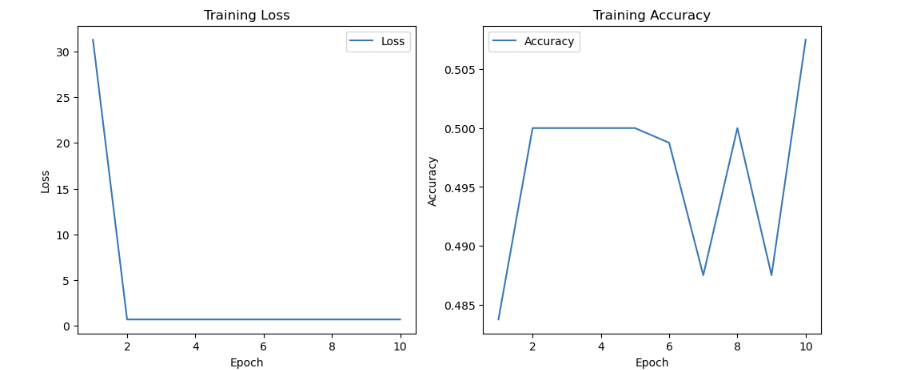
\includegraphics[width=15cm]{figuras/10 epocas.png}\\
	\autoria{Autoria Própria (2024)}
	\label{Fig:10epocas}
\end{figure}

Na Figura \ref{Fig:50epocas}, o treinamento foi realizado ao longo de 50 épocas com hiperparâmetros ajustados: tamanho do lote de 96 e taxa de aprendizado de 0,0005. Nesse experimento, observou-se uma melhora no desempenho em relação ao primeiro teste. O gráfico de erro apresentou uma diminuição mais acentuada, indicando que o modelo estava aprendendo de forma mais eficiente. O gráfico de acurácia também mostrou um aumento gradual, embora os valores ainda não tenham alcançado níveis desejáveis.

\begin{figure}[!h]
	\centering
	\caption{Treinamento ao longo de 50 épocas.}
	%\vskip 5mm
	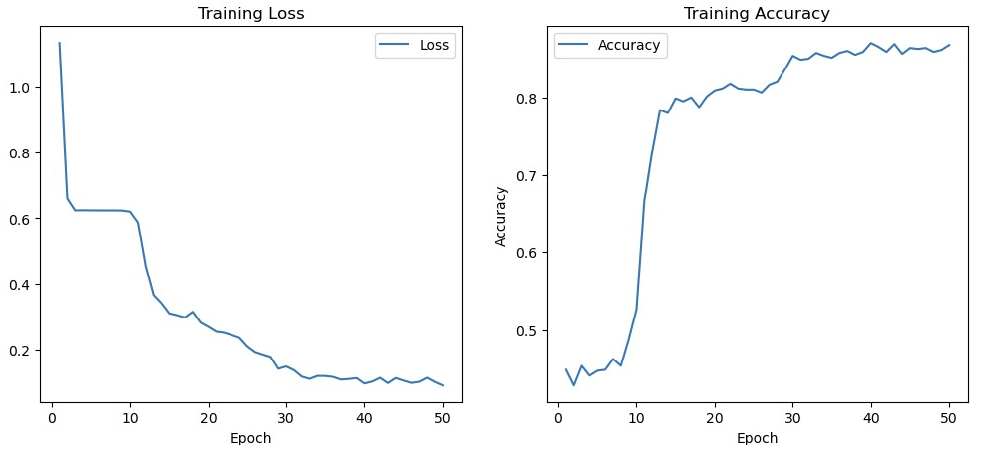
\includegraphics[width=14.4cm]{figuras/50 epocas.png}\\
	\autoria{Autoria Própria (2024)}
	\label{Fig:50epocas}
\end{figure}

Por fim, a Figura \ref{Fig:100epocas} apresenta o desempenho do modelo otimizado, treinado ao longo de 100 épocas. Os hiperparâmetros ajustados para este experimento foram um tamanho de lote de 120 e uma taxa de aprendizado de 0,0005. Com essas configurações, o modelo alcançou uma melhoria significativa em comparação aos experimentos anteriores. O gráfico de erro demonstrou uma redução contínua e mais pronunciada, indicando uma maior eficiência no ajuste do modelo aos dados. O gráfico de acurácia revelou um aumento consistente, com a acurácia final atingindo níveis bastante satisfatórios.


\begin{figure}[!h]
	\centering
	\caption{Treinamento ao longo de 100 épocas.}
	%\vskip 5mm
	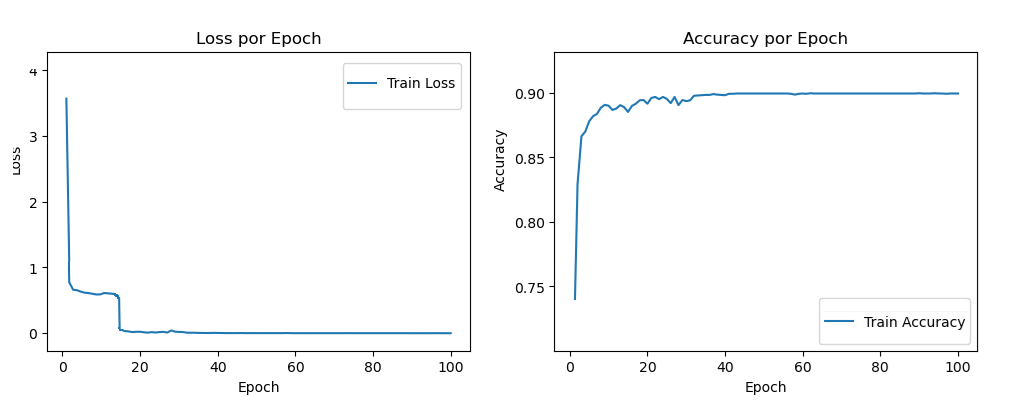
\includegraphics[width=15cm]{figuras/100 epocas.png}\\
	\autoria{Autoria Própria (2024)}
	\label{Fig:100epocas}
\end{figure}

 A \ac{MC} da Figura \ref{Fig:100Matriz} demonstra o desempenho do melhor modelo de classificação, apresentando a distribuição dos casos de verdadeiros e falsos positivos e negativos. O quadrante superior esquerdo indica que o modelo classificou corretamente 235 casos de SIGATOKA, enquanto o quadrante superior direito indica que classificou incorretamente 165 casos. No quadrante inferior esquerdo, estão os casos de falso positivo, ou seja, o modelo classificou incorretamente 18 imagens saudáveis como SIGATOKA. Por fim, no quadrante inferior direito, o modelo classificou corretamente 382 casos de folhas saudáveis.

Analisando a matriz de confusão, é possível notar que o modelo apresenta um bom desempenho. Caso contrário, é mais fácil identificar quais classes estão apresentando dificuldades, permitindo ajustar os hiperparâmetros ou explorar estratégias para melhorar a performance geral do modelo.

 
No entanto, é necessário resaltar que o desafio se dar pela demora no processo de aprendizado. Cada ajuste nos parâmetros exige um tempo considerável para completar novamente o treinamento, sendo que, o resultado de cada iteração leva por cerca de 3 horas. Isso pode tornar o processo de otimização lento e custoso, especialmente quando são necessários múltiplos testes.

\begin{figure}[!h]
	\centering
	\caption{Matriz de confusão}
	%\vskip 5mm
	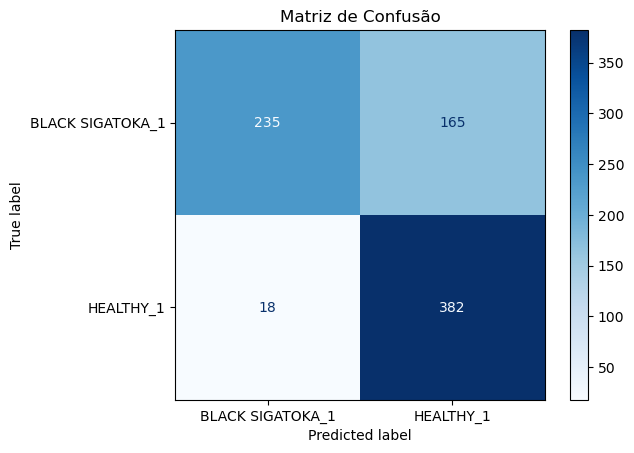
\includegraphics[width=10cm]{figuras/100 epocMatriz.png}\\
	\autoria{Autoria Própria (2024)}
	\label{Fig:100Matriz}
\end{figure}


\section{CONSIDERAÇÕES FINAIS E CRONOGRAMA}

O sistema proposto neste trabalho busca identificar problemas na plantação de bananeiras. Dessa forma, foi projetado um classificador baseado eme redes neurais convolucionais para processamento de imagens e detecção de doenças na cultura avaliada. Inicialmente,  projetou-se um classificador binário (apenas duas classes), em que considerou-se a folha da bananeira sem a doença e com a sigatoka (considerada a doença mais destrutiva da cultura da bananeira). Resultados encontrados mostraram-se promissores, embora, apresente necessidades de ajustes no sistema projetado a fim de otimizar os resultados de classificação. Assim, para etapa seguinte, pretende-se utilizar etapas de pré e pró processamento, além de avaliar outras doenças, gerando um classificador de multiplas classes. 

Neste contexto, para dar continuidade ao trabalho deve-se desenvolver as atividades previstas no quadro~\ref{tab:q2}, distribuídas conforme complexidade, eventos e tempo necessário para conclusão de cada etapa, e assim finalizando o trabalho. 


%colocar a tabela na página de cima
\begin{quadro}[!htb]
%\caption{Principais referências bibliográficas consultadas} \label{tab:q1}\\
\caption{Cronograma das atividades que serão realizadas durante o projeto.}\label{tab:q2}
\centering
\begin{tabular}{|p{45 mm }|c|c|c|c|c|c|}

\hline \centering \textbf{\footnotesize Atividades Previstas}   & \textbf{\footnotesize Out}  & \textbf{\footnotesize Nov} & \textbf{\footnotesize Dez} & \textbf{\footnotesize Jan} & \textbf{\footnotesize Fev} & \textbf{\footnotesize Mar} \\
\hline  Revisão bibliográfica&   x & x &  &  & &    \\ 
\hline  Preparar mais dados para inspeção & x & x  &  &  &  &   \\ 
\hline Ajustar a rede neural para novas doenças;  &   &  x &  &  &  &\\ 
\hline  Treinamento a rede neural convolucional;   &  &  & x & x &  &  \\
\hline  Identificar doenças do cultivo da banana   &  &  & x & x &  &  \\ 
\hline Analisar a acurácia e a taxa de erro da rede neural;     &  &  &  & x & x &    \\ 
%\hline Fazer a avaliação dos dados obtidos durante o experimento   &  &  & x & x &    \\  
\hline  Redigir TCC   &  &  &  & x & x & x  \\
\hline  Defender TCC   &  &  &  &  &  & x  \\
\hline 
\end{tabular}
\end{quadro}


% Nesta seção serão apresentados os resultados dos testes para validação do trabalho. Cada módulo do sistema foi testado separadamente, de acordo com sua funcionalidade, em seguida foram realizados testes do sistema funcionado integralmente, aplicado ao protótipo de estufa. 


% \section{Módulo sensores}

% Para validar o módulo de sensores, foram realizados testes específicos para cada grandeza medida pelos sensores. Foram testados valores compreendidos na Tabela \ref{tab:my-tablex}, objetivando-se alcançar os extremos de cada grandeza. 

% \subsection{Testes de temperatura}

% Com o sensor de temperatura conectado ao circuito de condicionamento de sinais, foram realizados testes em laboratório. Foram medidos valores e comparados com medidas realizadas com termômetro digital. A primeira medida foi realizada em um congelador, onde foi possível constatar que o sensor é capaz de aferir temperaturas negativas. Foram realizados testes à temperatura ambiente, como apresentado na Figura \ref{fig:testetemp}, onde o valor coincidiu com o termostato do controle do ar-condicionado.

% \begin{figure}[!h]
% 	\centering
% 	\caption{Estado da bomba submersa}
% 	%\vskip 5mm
% 	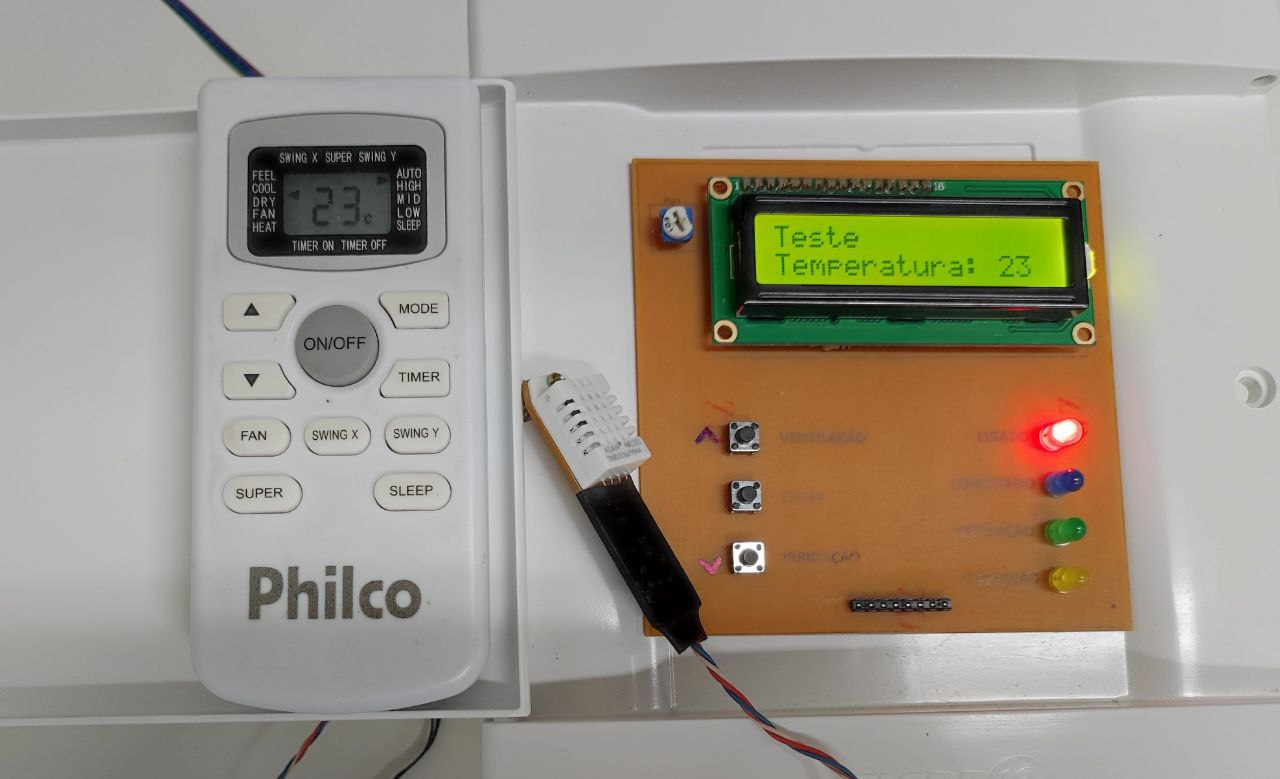
\includegraphics[width=12cm]{figuras/testetemp.jpg}\\
% 	\autoria{Autoria Própria}
% 	\label{fig:testetemp}
% \end{figure}

% Foram realizados testes em outros ambientes, resultando em dados aproximados da temperatura real. Dessa forma, o sensor DHT-22 apresentou resultados satisfatórios e condizentes com a aplicação, com suas variações estando dentro da faixa estabelecida na folha de dados do sensor.

% \subsection{Testes de umidade do ar}

% Por se tratar de uma grandeza difícil de controlar com os recursos presentes, foram realizados apenas teste de umidade relativa do ar em ambiente externo e interno, realizando múltiplas medidas e comparando a variação entre elas. A Tabela apresenta os resultados das medidas obtidas nos testes.

% \begin{table}[!h]
% \centering
% \caption{Medidas de umidade do ar em ambiente interno e externo}
% \label{tab:umidadear}
% \begin{tabular}{c|c|c}
% \hline
% Umidade do ar & Ambiente interno & Ambiente externo \\ \hline
% Medida 1 & 38.9\% & 34.7\% \\ \hline
% Medida 2 & 38.9\% & 34.6\% \\ \hline
% Medida 3 & 39.6\% & 34.7\% \\ \hline
% Medida 4 & 39.4\% & 35.2\% \\ \hline
% Medida 5 & 39.6\% & 35.3\% \\ \hline
% \end{tabular}
% \\
% \autoria{Autoria própria}
% \end{table}

% Analisando os dados apresentados, é possível observar uma baixa variação entre os valores de umidade relativa do ar, sendo a umidade medida em ambiente interno ligeiramente maior, por conta da presença de pessoas no local e baixa ventilação. Por conta da constância dos resultados, é possível afirmar que a confiabilidade do sensor está condizente com os requisitos do sistema. 

% \subsection{Testes de umidade do solo}
% Os testes de umidade do solo foram realizados em recipientes contendo variados tipos de terra e variando a quantidade de água presente. Primeiramente foi medido o valor obtido pelo sensor sem contato com o solo, como visto na Figura \ref{fig:avazio}. O valor esperado para o teste era de 0\%, sento obtido medida equivalente.

% \begin{figure}[!h]
% 	\centering
% 	\caption{Teste com sensor seco}
% 	%\vskip 5mm
% 	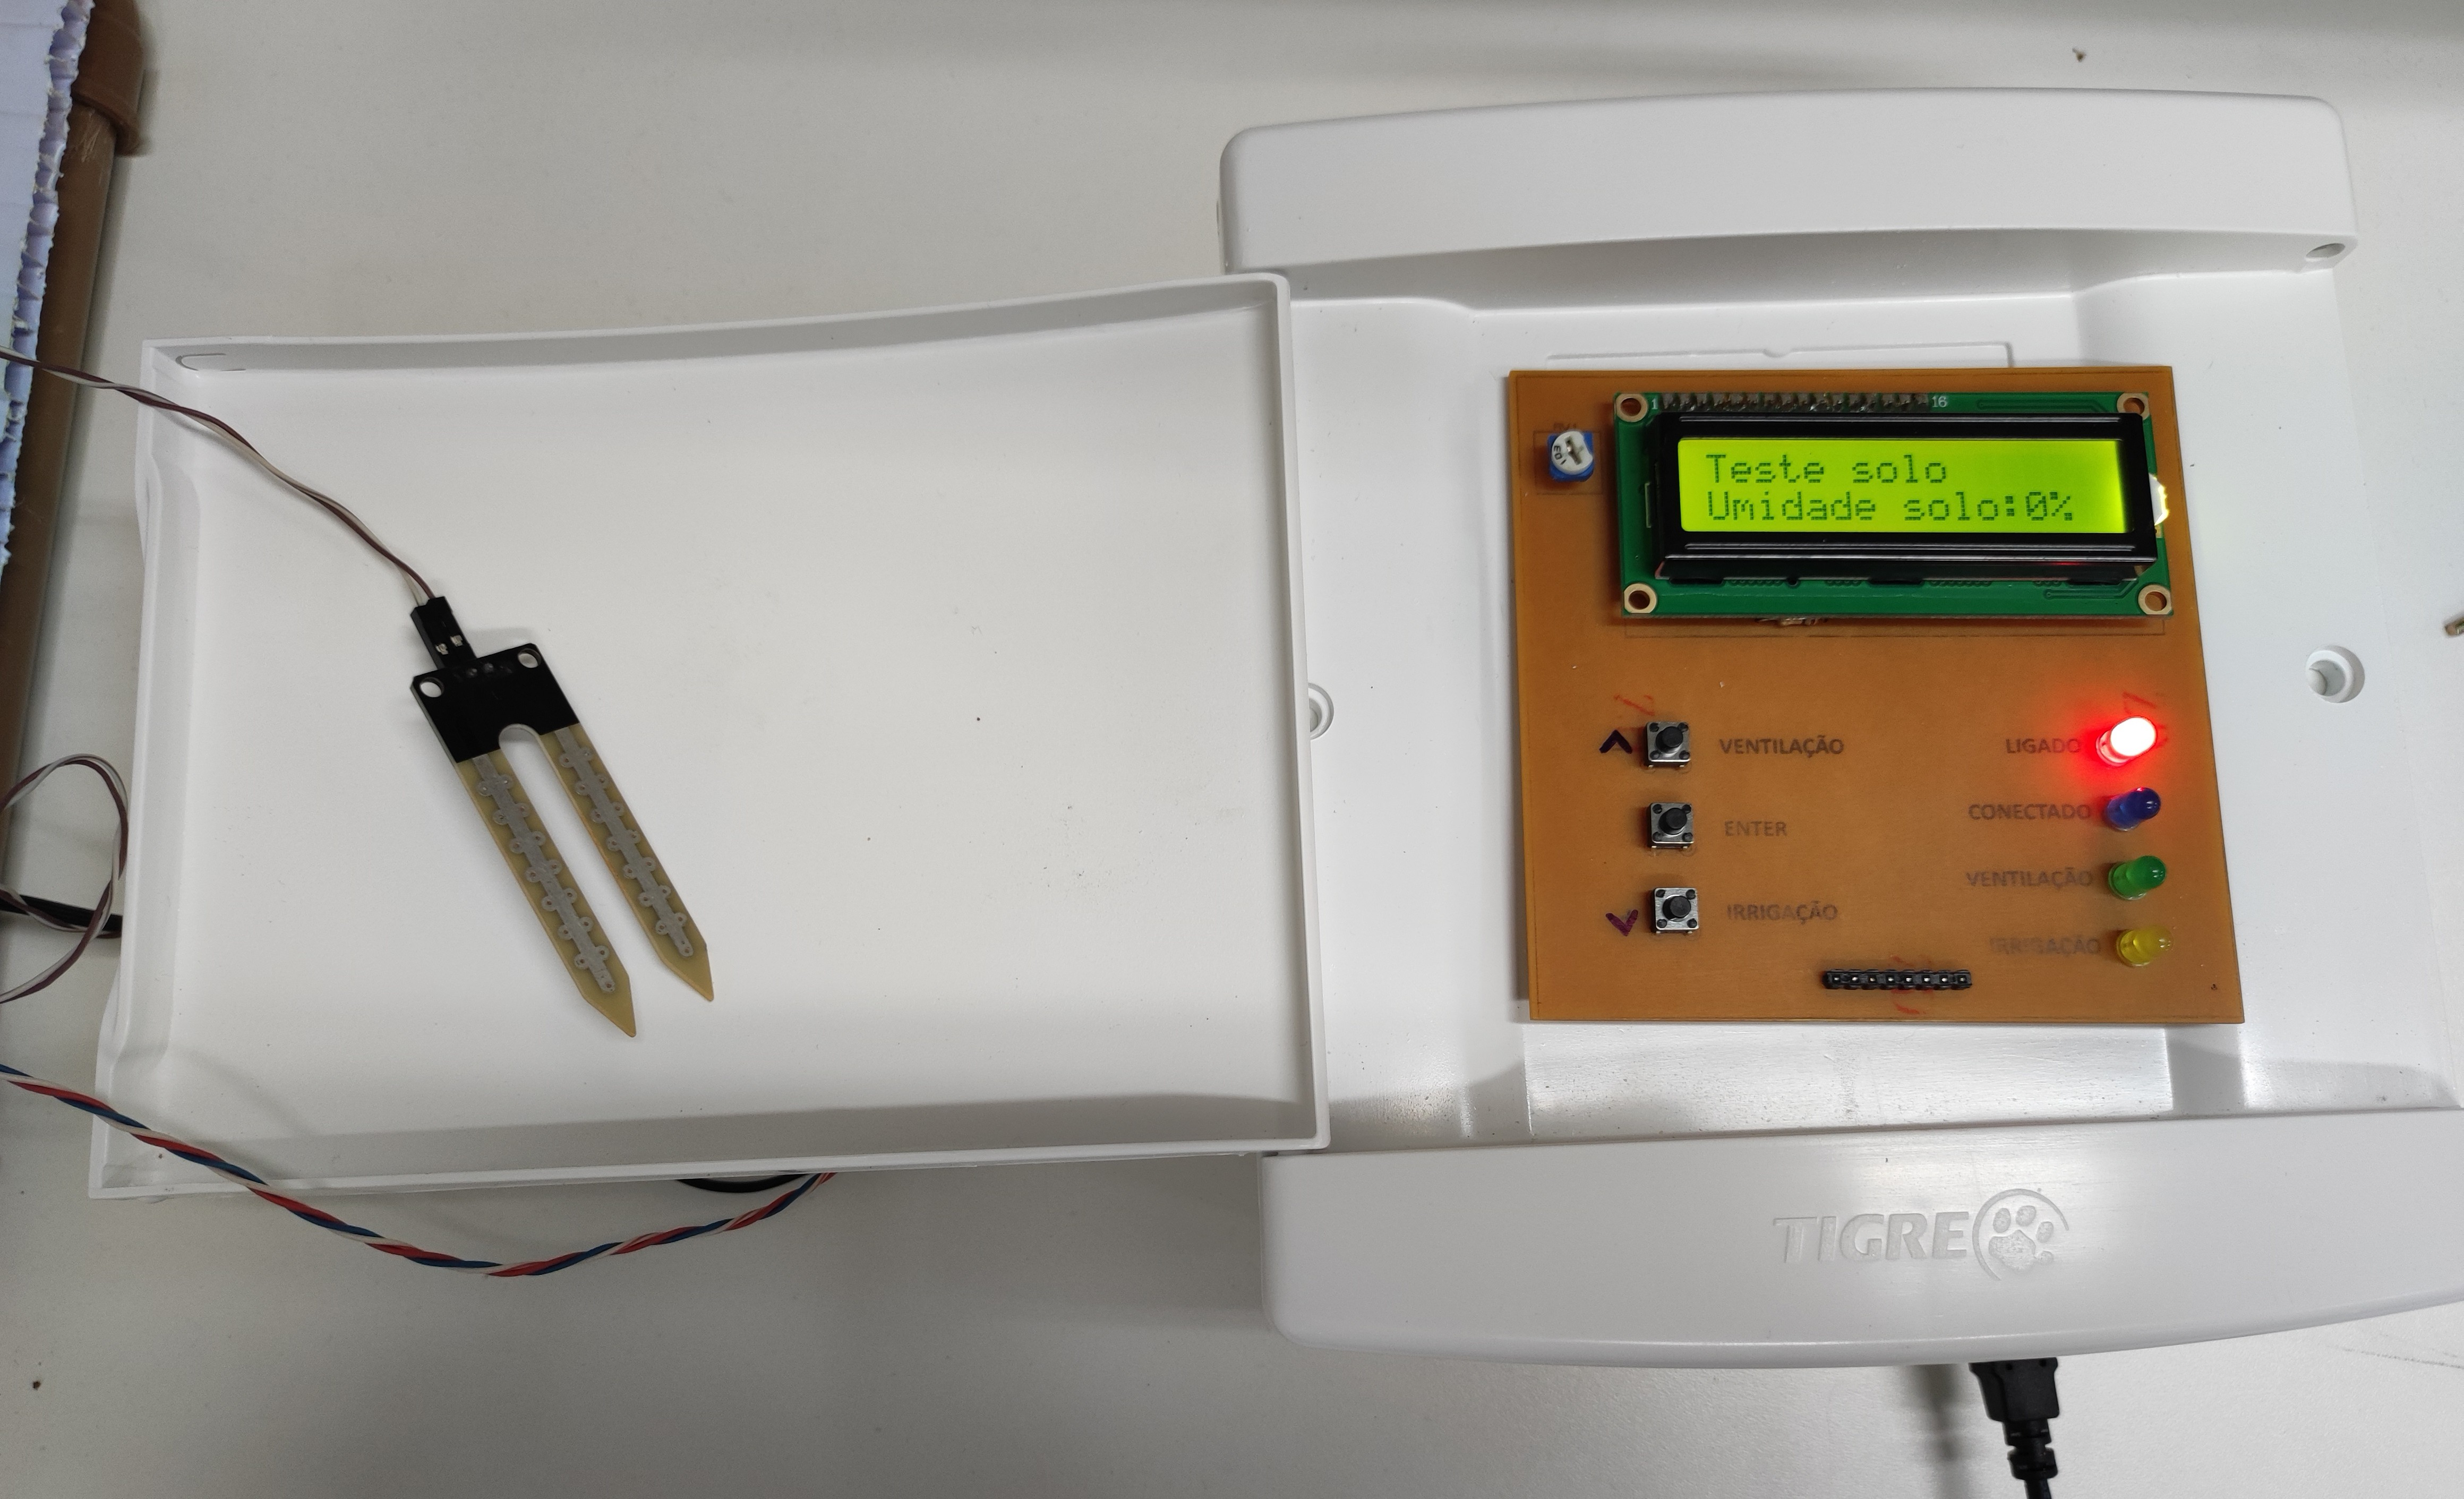
\includegraphics[width=8cm]{figuras/avazio.jpg}\\
% 	\autoria{Autoria Própria}
% 	\label{fig:avazio}
% \end{figure}

% O sensor foi testado em três tipos de solo, sendo eles arenoso, orgânico e argiloso, apresentados na Figura \ref{fig:solos}, que variam a forma com que absorvem a água. Inicialmente os três solos estavam totalmente secos durante a realização das medidas, desse modo, o sensor captou umidade do solo próximo a 0 para os três testes.

% \begin{figure}[!h]
% 	\centering
% 	\caption{Tipos de solo testados}
% 	%\vskip 5mm
% 	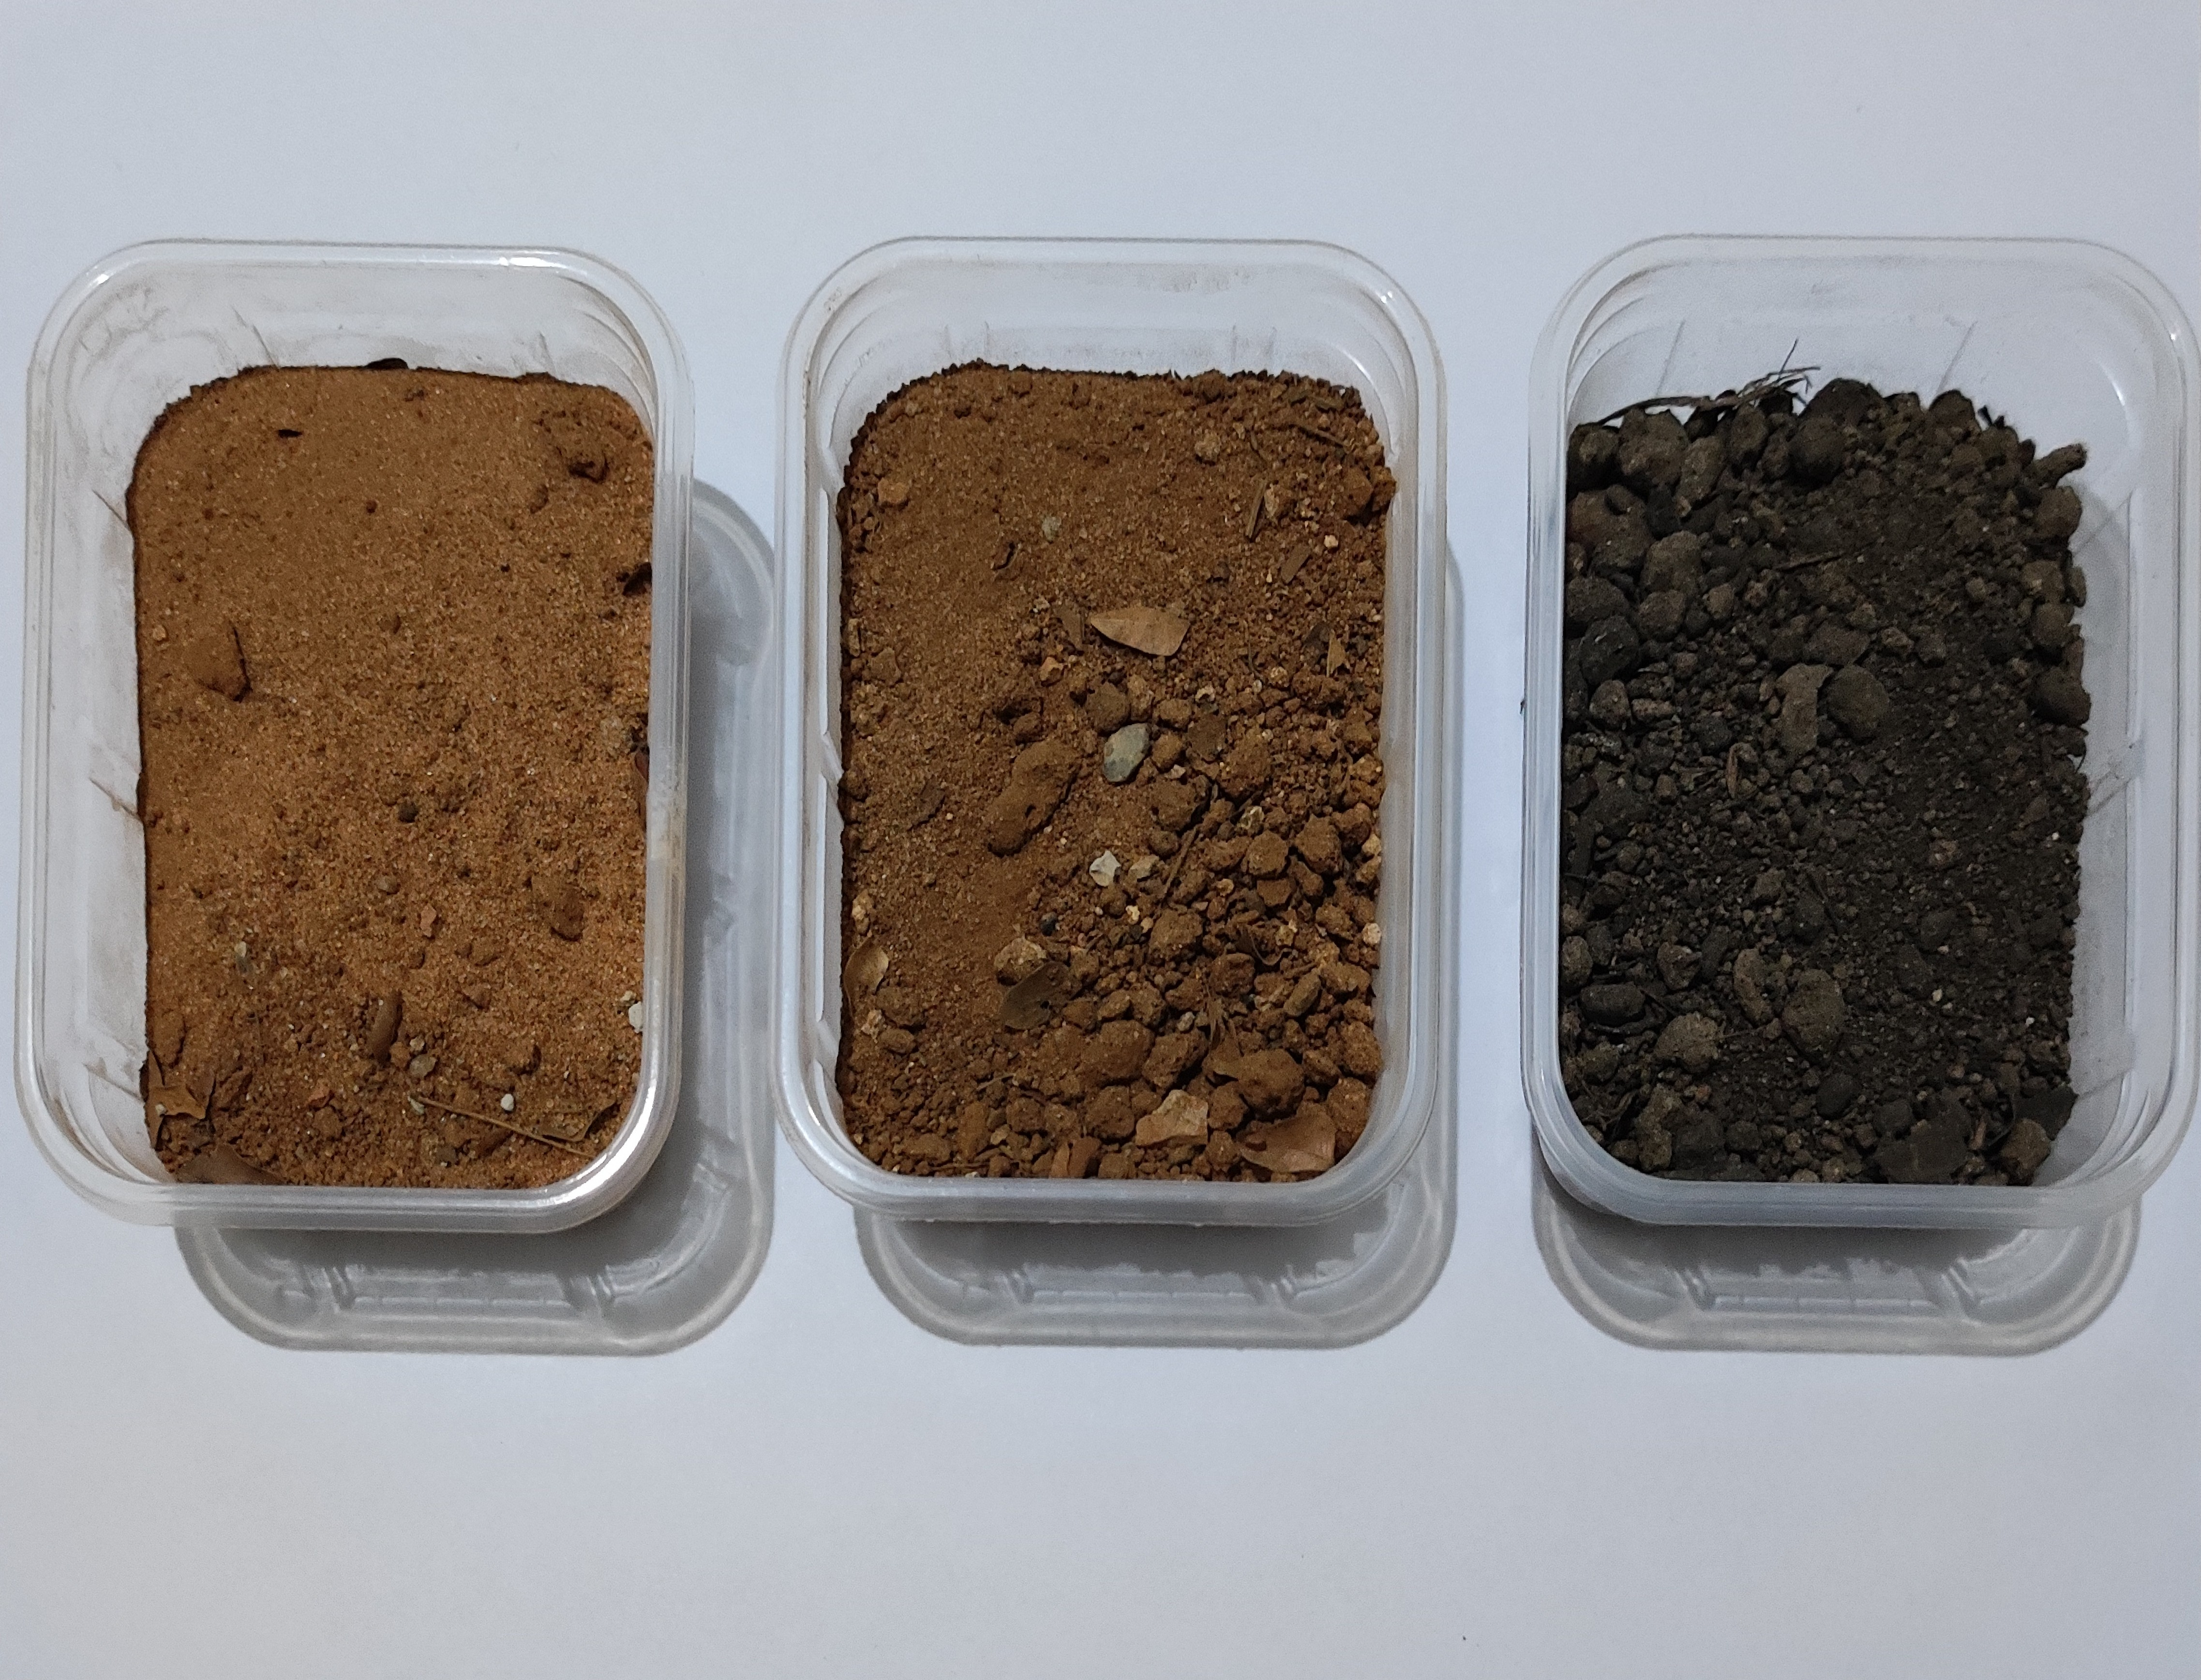
\includegraphics[width=8cm]{figuras/solos.jpg}\\
% 	\autoria{Autoria Própria}
% 	\label{fig:solos}
% \end{figure}

% Em seguida, foi adicionado cerca de 20ml de água nos três recipientes, e foram realizadas novas medidas. Nesse teste, a umidade do solo obtida variou conforme o tipo de solo, sendo que o solo arenoso apresentou maior valor de umidade, por conta da baixa absorção que esse tipo de solo apresenta. 

% Foi adicionado água gradativamente, até o limite da capacidade do recipiente, as medidas foram coletadas, os resultados das medidas foram organizados na Tabela \ref{tab:umidadesolo}. Em seguida o sensor foi mergulhado em água, onde o valor da umidade do solo se tornou 100\%, como esperado.

% \begin{table}[!h]
% \centering
% \caption{Medidas de umidade do solo em três tipos de solo}
% \label{tab:umidadesolo}
% \begin{tabular}{c|c|c|c}
% \hline
% \begin{tabular}[c]{@{}c@{}}Quantidade\\  de água\end{tabular} & \begin{tabular}[c]{@{}c@{}}Solo \\ arenoso\end{tabular} & \begin{tabular}[c]{@{}c@{}}Solo \\ orgânico\end{tabular} & Solo argiloso \\ \hline
% 0 & 0\% & 0\% & 0\% \\ \hline
% 20ml & 18\% & 14\% & 15\% \\ \hline
% 40ml & 39\% & 31\% & 34\% \\ \hline
% 60ml & 62\% & 55\% & 58\% \\ \hline
% 80ml & 85\% & 71\% & 76\% \\ \hline
% \end{tabular}
% \\
% \autoria{Autoria própria}
% \end{table}

% Analisando os dados apresentados, é possível afirmar que o sensor é adequado para a aplicação do presente trabalho, sendo capaz de medir a variação da umidade do solo para diferentes quantidades de água e para variados tipos de solo. 

% \section{Módulo atuador}

% O módulo relé utilizado como atuador neste trabalho permite grande versatilidade no acionamento de cargas, podendo acionar diretamente cargas em corrente contínua e corrente alternada de tensão monofásica, além de poder acionar indiretamente cargas trifásicas, fazendo parte do circuito de controle. Desse modo, os testes para o módulo atuador consistiram em acionar um motor de corrente contínua e um motor de indução trifásico, apresentados na Figura \ref{fig:motores}. 

% \begin{figure}[!h]
% 	\centering
% 	\caption{Testes com motor trifásico e motor de corrente contínua}
% 	%\vskip 5mm
% 	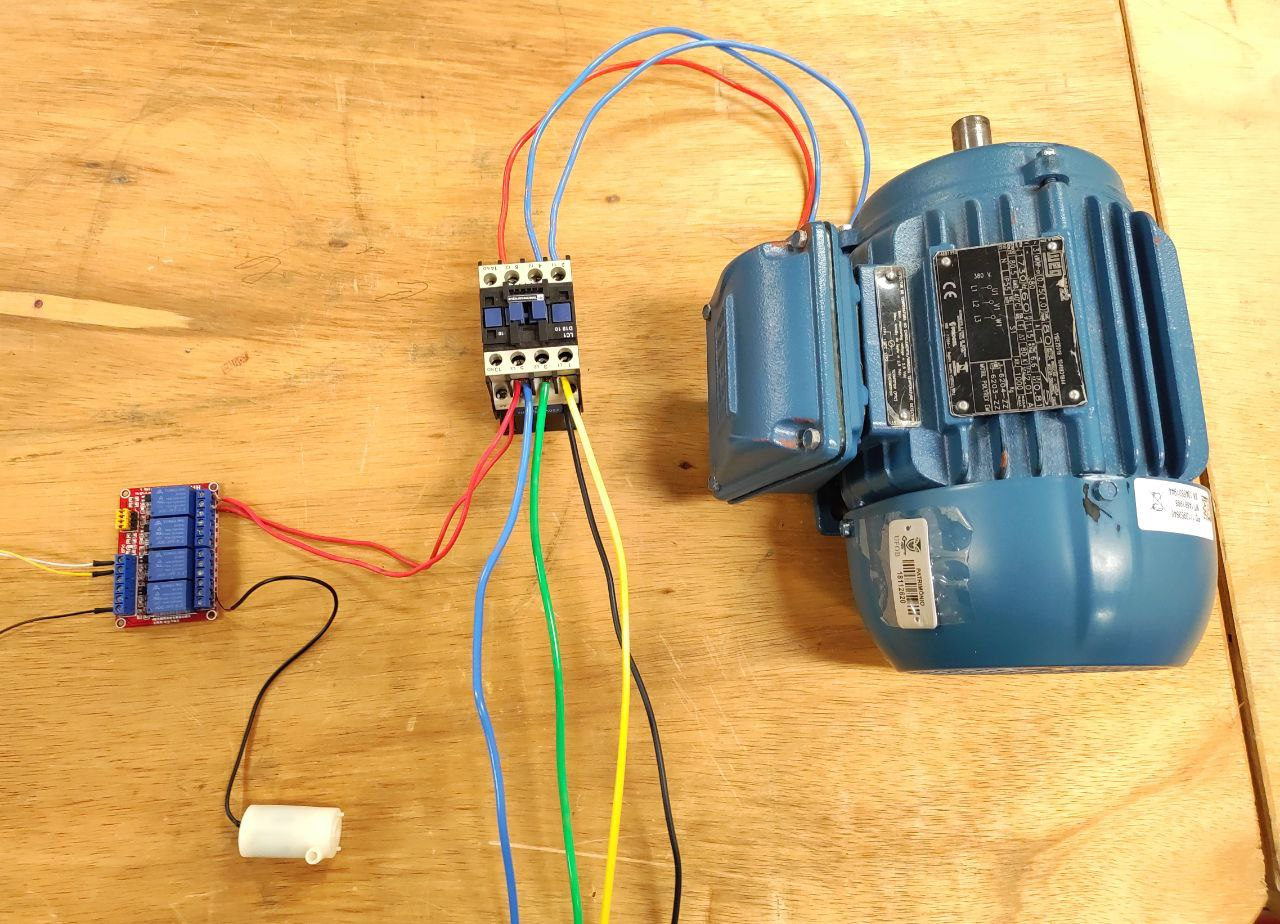
\includegraphics[width=9cm]{figuras/motores.jpg}\\
% 	\autoria{Autoria Própria}
% 	\label{fig:motores}
% \end{figure}

% Para acionar o motor em corrente contínua, foi ligado o terminal positivo de uma fonte de 12V no pino normalmente aberto do relé, o fio positivo do motor foi ligado no pino comum do relé e o fio negativo do motor foi ligado diretamente ao terminal negativo da fonte, como visto no esquema de ligação apresentado na Figura \ref{fig:motorcc}.

% \begin{figure}[!h]
% 	\centering
% 	\caption{Diagrama elétrico de ligação para o motor corrente contínua}
% 	%\vskip 5mm
% 	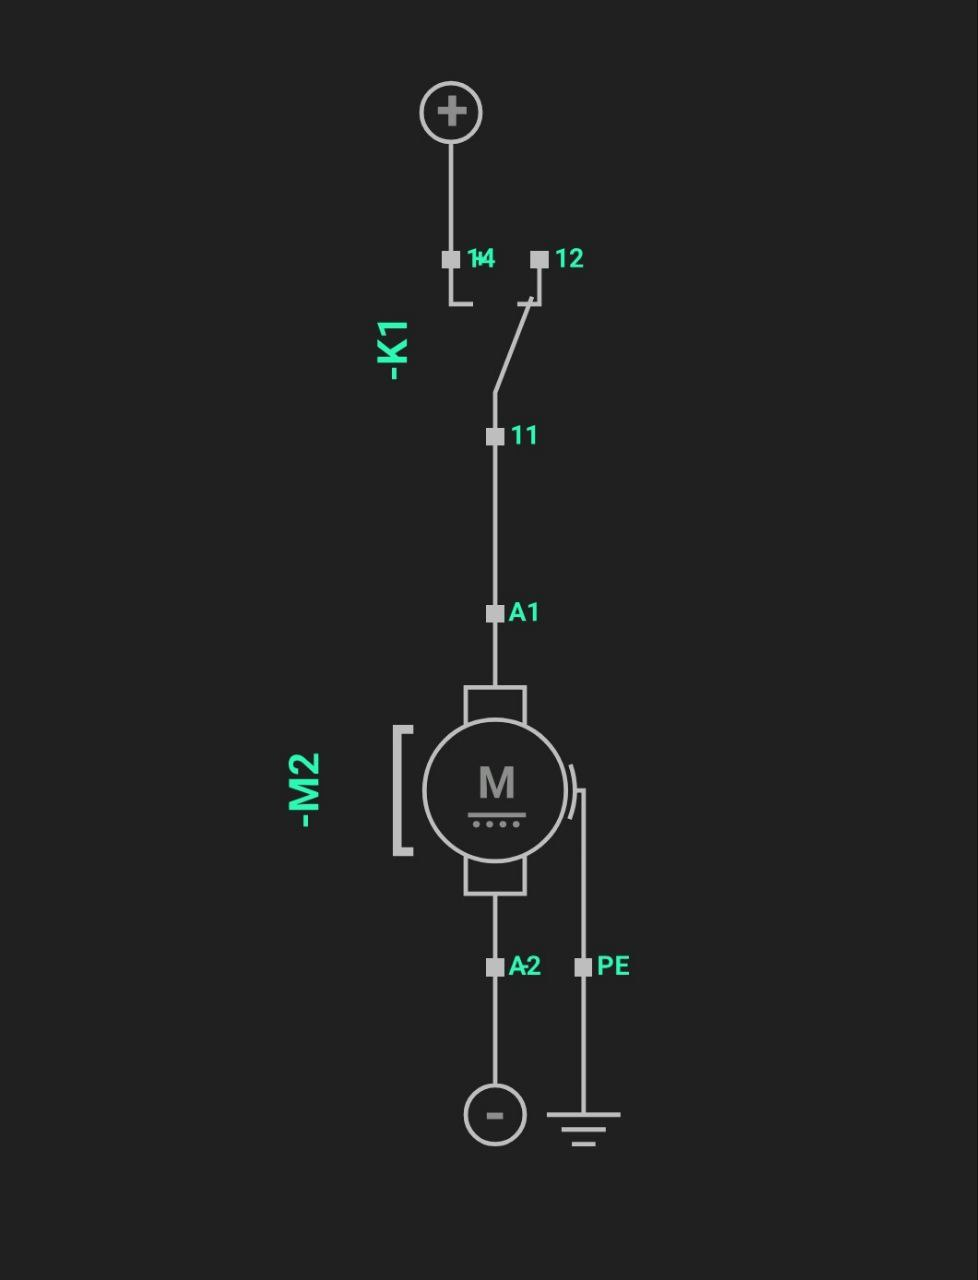
\includegraphics[width=6cm]{figuras/motorcc.jpg}\\
% 	\autoria{Autoria Própria}
% 	\label{fig:motorcc}
% \end{figure}

% O teste de acionamento do motor trifásico foi realizado com o auxílio de um contator, onde o relé foi responsável pelo acionamento da bobina do contator, que por sua vez, acionou o motor trifásico, o esquema de ligação é apresentado na Figura \ref{fig:motorca}.

% \begin{figure}[!h]
% 	\centering
% 	\caption{Diagrama elétrico de ligação para o motor trifásico}
% 	%\vskip 5mm
% 	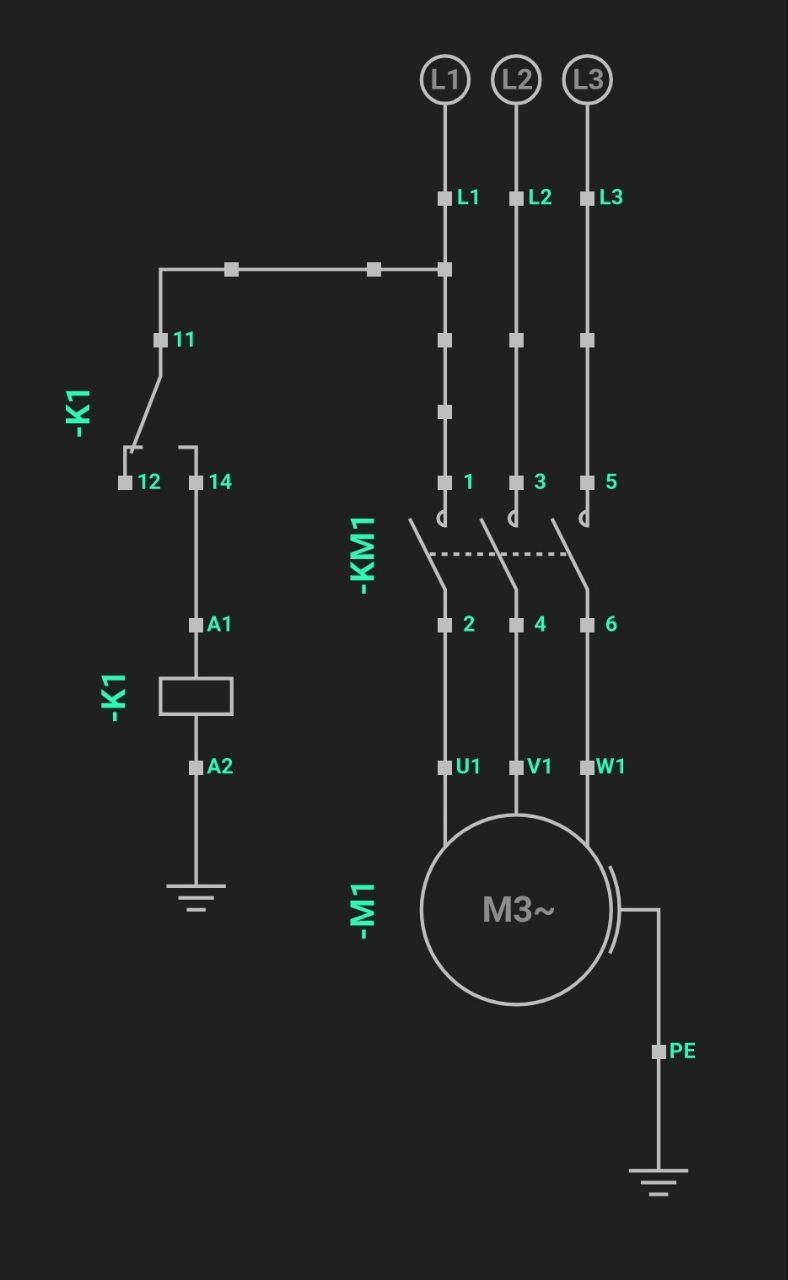
\includegraphics[width=6cm]{figuras/motorca.jpg}\\
% 	\autoria{Autoria Própria}
% 	\label{fig:motorca}
% \end{figure}

% Em ambos os testes foi possível acionar os motores, podendo estes atuar como bombas de irrigação e de ventilação, em pequena e grande escala. Desse modo, o módulo atuador se mostrou eficaz, acionando de maneira rápida e segura as cargas testadas, sedo adequada a sua utilização no projeto.

% \section{Circuito de condicionamento de sinais}

% O circuito de condicionamento de sinais teve seu desempenho testado paralelamente aos testes dos sensores, porém, foram realizados testes específicos para averiguar outras características do seu funcionamento julgadas essenciais para o bom desempenho do sistema como um todo. 

% Ao coletar as informações dos sensores, o circuito tinha como primeira função converter os dados em valores que pudessem ser interpretados e comparados pelo resto do código e pelo usuário. Ao realizar os testes com o sensor de umidade do solo, o circuito de condicionamento de sinais foi capaz de converter o valor analógico enviado pelo sensor em um valor digital em escala decimal, que pôde ser exibido no visor da interface humano/máquina e usado para validação do sensor. 

% Para os teste de temperatura e umidade relativa do ar, o circuito de condicionamento de sinais foi capaz de executar todas as funções cruciais para o funcionamento do sensor DHT-22, sendo capar de interpretar o valor binário de 16 bits enviado pelo sensor e separar os dados de temperatura e umidade do ar, além de converte-los em escala decimal e exibir na IHM. 

% Graças ao bom funcionamento deste circuito, todos os testes realizados entre os módulos foram possíveis, decretando este como o principal componente do sistema, sendo indispensável para o funcionamento do protótipo como um todo. Destarte, este circuito tem seu funcionamento continuado mesmo com a ausência de outros módulos do sistema, como exemplo a conexão via radiofrequência com o módulo central ou a comunicação com a internet, onde o módulo é capaz de funcionar normalmente coletando os dados dos sensores e controlando os atuadores, além de exibir as informações para o usuário por meio da IHM

% Mesmo com a ausência do módulo sensores, o circuito de condicionamento de sinais foi capaz de manter o sistema em funcionamento no modo manual, onde o usuário aciona a ventilação ou irrigação através da IHM. No teste da desconexão com o módulo atuador, o circuito manteve a coleta e envio dos dados dos sensores, mantendo sua funcionalidade como plataforma de monitoramento.

% Todos os teste de validação foram realizados considerando situações extremas, onde alguma parte do sistema teve seu funcionamento comprometido, no entanto, o circuito de condicionamento de sinais foi capaz de manter-se funcionando adequadamente, perdendo apenas a funcionalidade referente à parte desconectada do sistema. Devido a esses resultados, foram adotadas medidas visando manter o circuito de condicionamento de sinais seguro, sendo instalado dentro da caixa de disjuntores e fixado por meio de parafusos, em local inacessível ao usuário do sistema.

% \section{Comunicação por radiofrequência}

% Os testes realizados para validar a comunicação entre o circuito de condicionamento de sinais e o módulo central, que foi realizada através de módulos de radiofrequência consistiu em estabelecer a comunicação e distanciar os módulos até que a comunicação fosse perdida. Foram realizados testes com dois modelos de módulos de radiofrequência diferentes, utilizando antenas diferentes. 

% No primeiro teste, os módulos foram posicionados lado a lado, com o objetivo de estabelece a conexão entre eles, o primeiro modelo testado, apresentado na Figura \ref{fig:hc12}, não estabeleceu conexão, se tornando inutilizável no projeto, os motivos para esse resultado podem estar ligados à uma falsificação dos módulos, já que outros trabalhos foram desenvolvidos com esse mesmo modelo e obtiveram bons resultados de conexão e distancia de transmissão de dados. 

% \begin{figure}[!h]
% 	\centering
% 	\caption{Primeiro modelo de módulo radiofrequência}
% 	%\vskip 5mm
% 	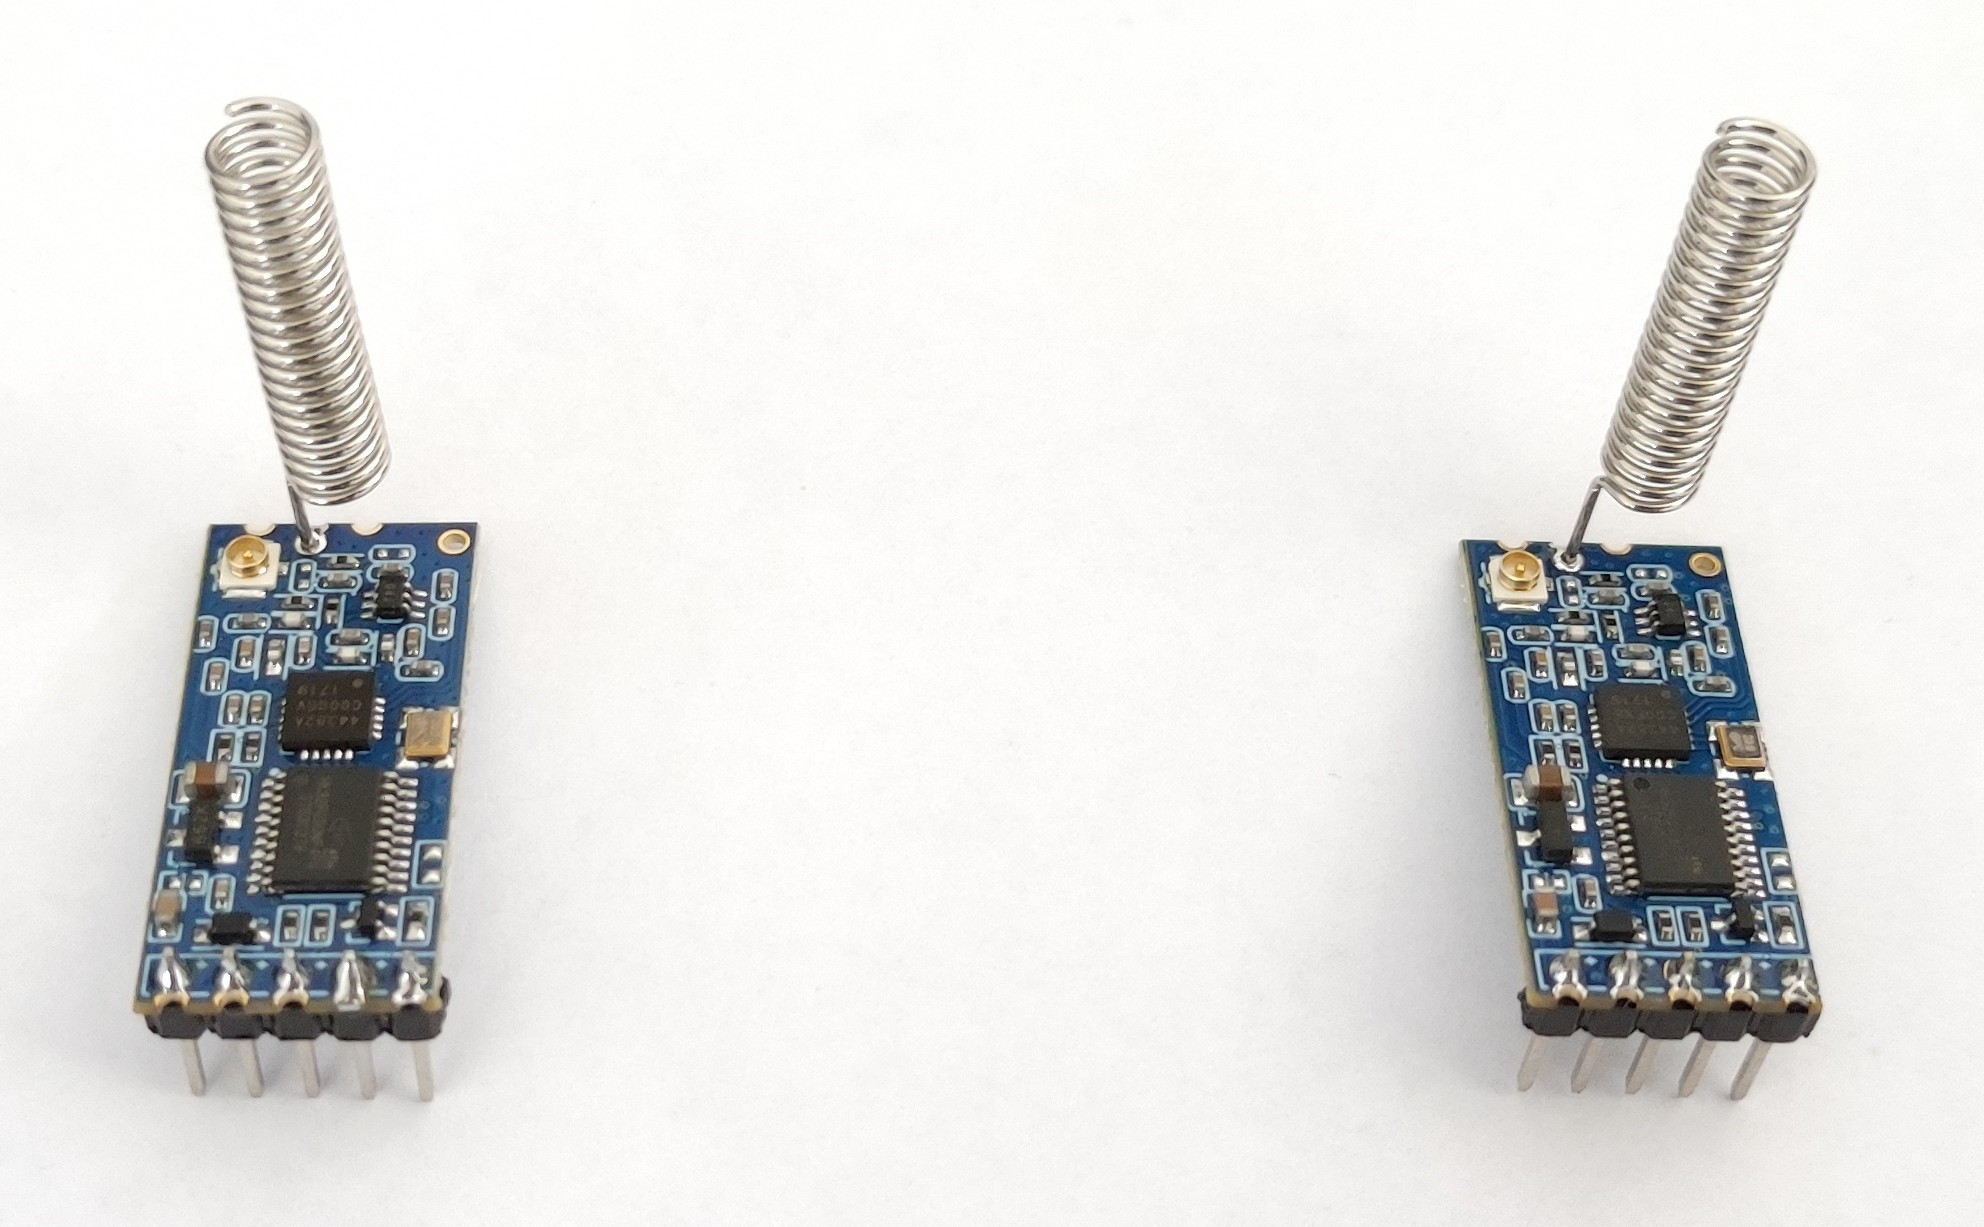
\includegraphics[width=10cm]{figuras/hc12.jpg}\\
% 	\autoria{Autoria Própria}
% 	\label{fig:hc12}
% \end{figure}

% Para o segundo modelo, apresentado na Figura \ref{fig:modrf}, o teste de estabelecimento de conexão obteve êxito, sendo possível transmitir dados entre os módulos. O segundo teste consistiu em distanciar os transmissores em 5 metros e testar a comunicação. Novamente, o segundo módulo conseguiu transmitir os dados entre o circuito de condicionamento de sinais e o módulo central. 

% \begin{figure}[!h]
% 	\centering
% 	\caption{Segundo modelo de módulo radiofrequência}
% 	%\vskip 5mm
% 	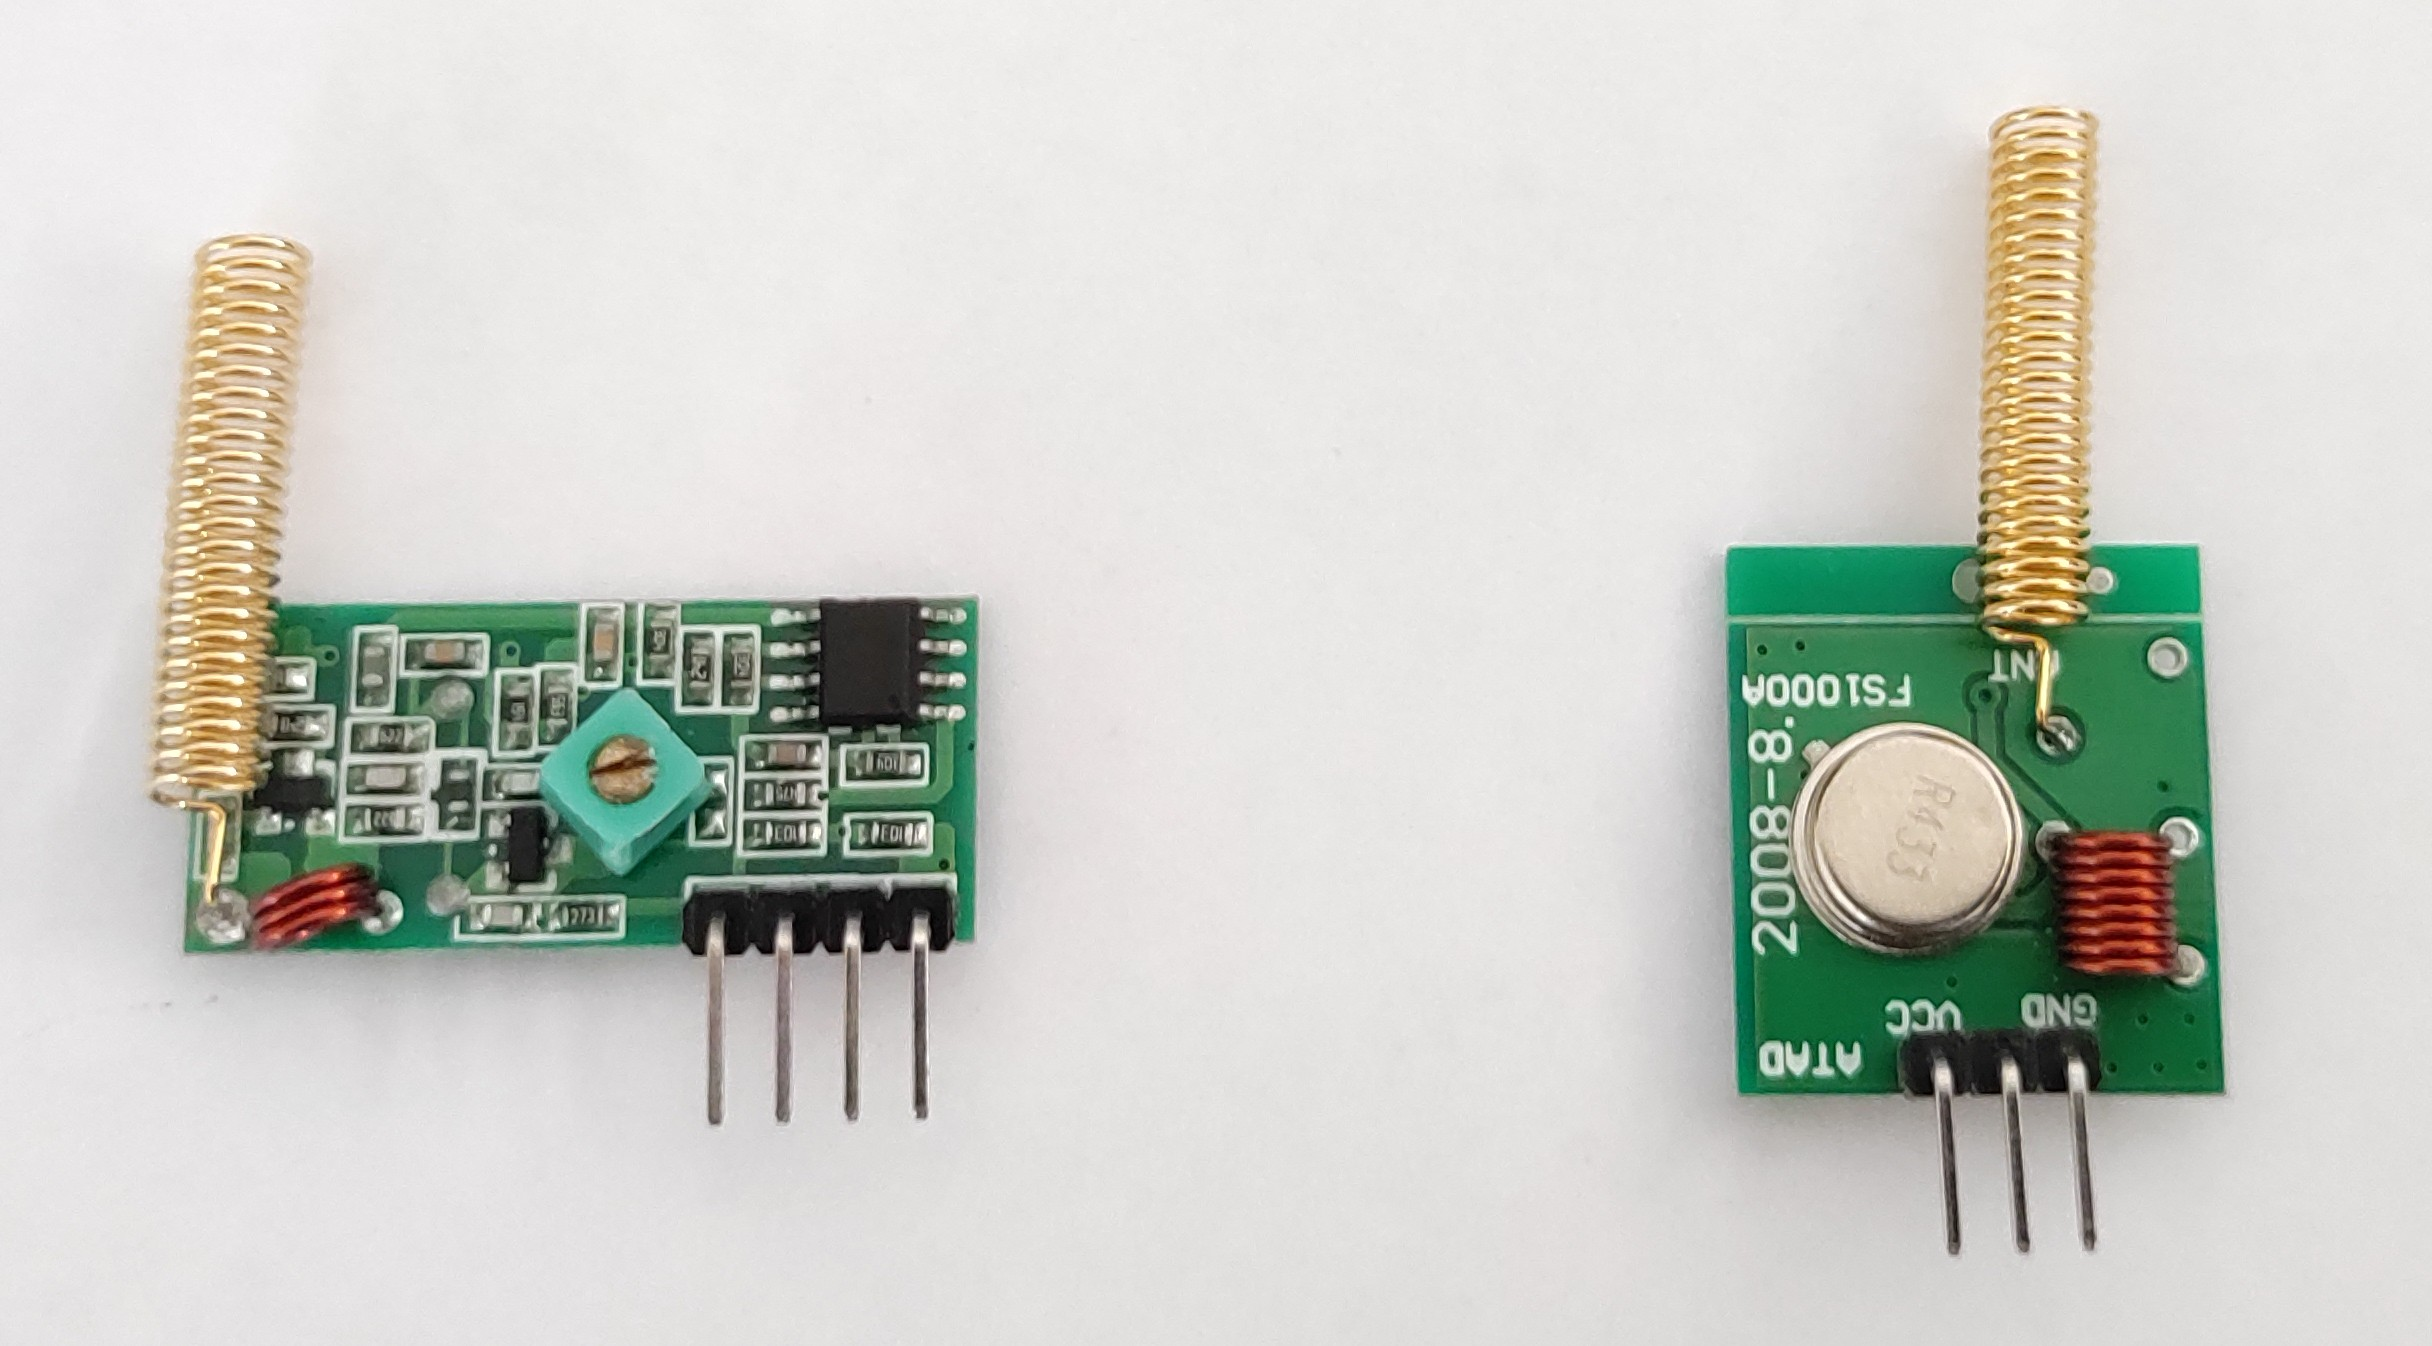
\includegraphics[width=8cm]{figuras/modrf.jpg}\\
% 	\autoria{Autoria Própria}
% 	\label{fig:modrf}
% \end{figure}

% No terceiro teste, os módulos foram separados em 10 metros. Nesta distancia, a comunicação apresentou falhas, onde nem todos os dados enviados pelo circuito de condicionamento de sinais eram recebidos pelo módulo central. O quarto teste consistiu em separar os transmissores em 15 metros, nessa distância a conexão entre os módulos foi perdida. 

% Os resultados obtidos para o segundo modelo de módulo foram como o esperado, considerando as características do transmissor e da antena utilizada. Caso a antena fosse substituída por uma maior, a distância de comunicação poderia ser estendida para cerca de 50 metros. Por conta da baixa distância de transmissão alcançada, optou-se por instalar o módulo central no mesmo recipiente que o circuito de condicionamento de sinais, aproveitando a mesma fonte de alimentação para todo o sistema. Desse modo, todo o sistema pode ser instalado no mesmo ambiente, vale ressaltar que esse resultado não comprometeu o funcionamento do protótipo.

% \section{Módulo central}

% O módulo central tem como principal objetivo intermediar a comunicação entre o sistema e a internet. Por meio deste, é possível acessar as informações do plantio de qualquer lugar do mundo que tenha acesso à internet. Foram realizados testes de conectividade e comunicação através do protocolo MQTT. O protocolo foi implementado no ESP32, por conta do seu módulo wi-fi, sendo conectado à internet e estabelecido contato com o \textit{broker}, em seguida, foi acessado o aplicativo na mesma rede wi-fi em que o módulo central estava conectado e a comunicação foi estabelecida com sucesso. 

% Outros testes foram realizados, sendo eles o acesso ao aplicativo usando uma rede wi-fi diferente da que o módulo central estava conectado e o acesso usando os dados móveis de internet do celular. Em ambos os testes a comunicação foi estabelecida, como apresentado na Figura \ref{fig:telas}.

% \begin{figure}[!h]
% 	\centering
% 	\caption{Comunicação entre o aplicativo}
% 	%\vskip 5mm
% 	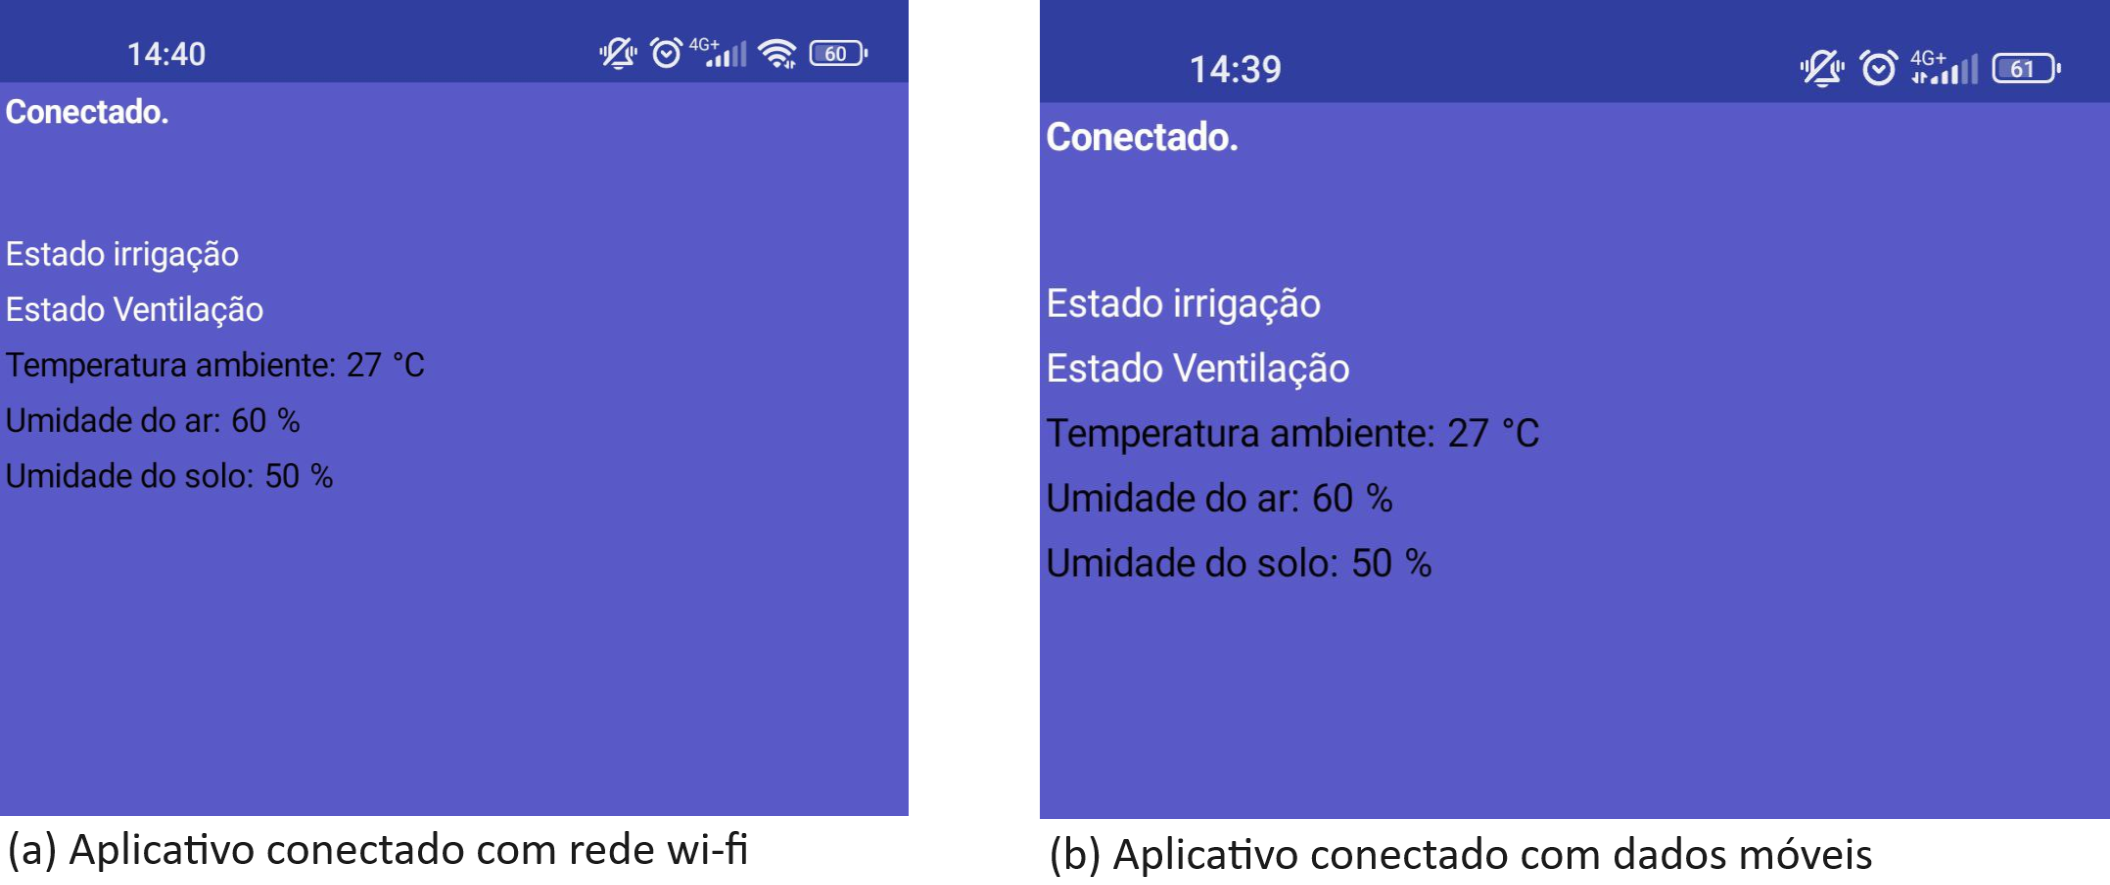
\includegraphics[width=13cm]{figuras/telas.png}\\
% 	\autoria{Autoria Própria}
% 	\label{fig:telas}
% \end{figure}

% Analisando o resultado dos teste, é possível observar que o protocolo MQTT permite uma conexão segura e facilitada, tendo um excelente potencial em aplicações de IoT, permitindo um número ilimitado de dispositivos conectados ao \textit{broker} e possibilitando um tráfego seguro de dados. 

% \section{Teste Prático}

% O protótipo final do trabalho foi montado em uma caixa de disjuntores anti-chamas, com os componentes fixados com parafusos. Todas as conexões entre os módulos foram realizadas dentro da caixa, de maneira que o usuário final não tenha acesso, o processo de montagem é apresentado na Figura \ref{fig:montagem}. 

% \begin{figure}[!h]
% 	\centering
% 	\caption{Montagem do trabalho}
% 	%\vskip 5mm
% 	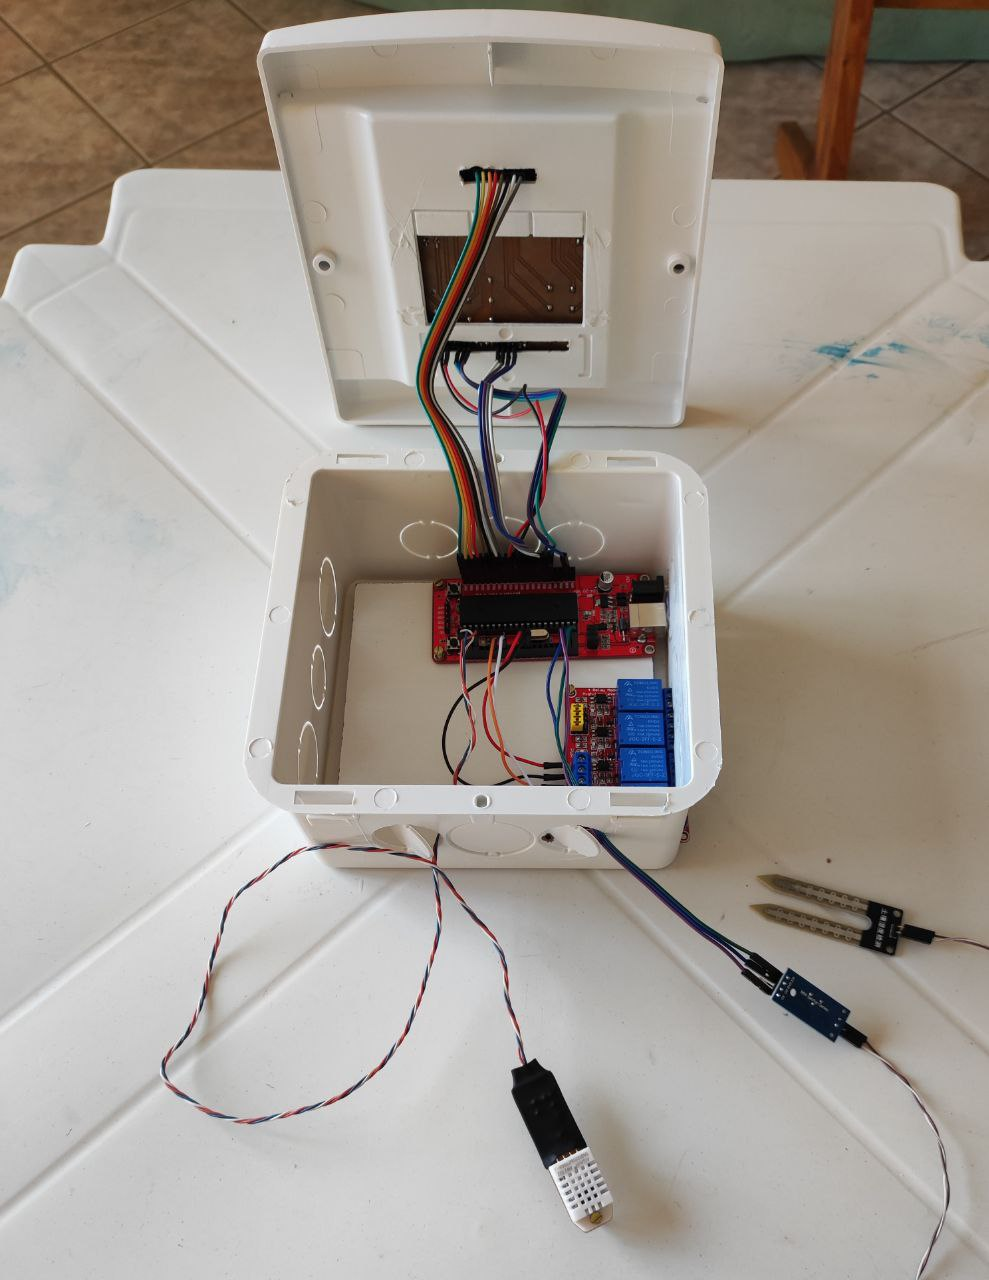
\includegraphics[width=6cm]{figuras/montagem.jpg}\\
% 	\autoria{Autoria Própria}
% 	\label{fig:montagem}
% \end{figure}

% Os módulos foram posicionados de maneira que posse possível a conexão externa dos atuadores e alimentação do sistema. Desse modo, fica disponível ao usuário todas as conexões necessárias para o funcionamento do sistema. Na Figura \ref{fig:releco} são apresentadas as portas de conexão entre o módulo relé e as cargas, tendo seus parafusos de fixação em fácil acesso pelo usuário.

% \begin{figure}[!h]
% 	\centering
% 	\caption{Conexões externas do sistema}
% 	%\vskip 5mm
% 	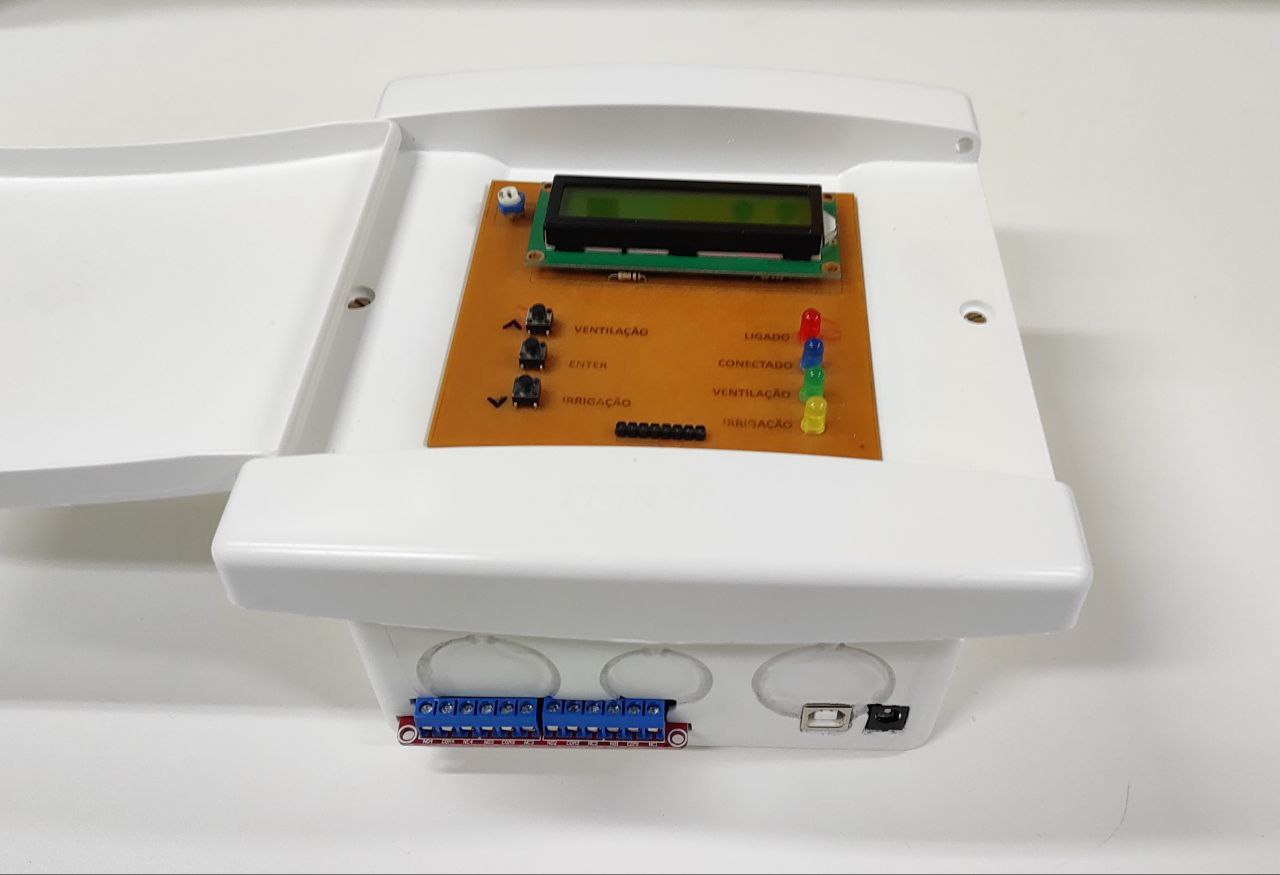
\includegraphics[width=7cm]{figuras/releco.jpg}\\
% 	\autoria{Autoria Própria}
% 	\label{fig:releco}
% \end{figure}

% Os sensores foram conectados internamente ao circuito de condicionamento de sinais e saíram da caixa através de passagens laterais, conforme Figura \ref{fig:saidasensores}.  Desse modo, os sensores podem ser posicionados de acordo com a necessidade do usuário. A maneira com que foi posicionada a saída dos sensores inibe que água escorra para dentro da caixa, protegendo o circuito interno.

% \begin{figure}[!h]
% 	\centering
% 	\caption{Saída dos sensores}
% 	%\vskip 5mm
% 	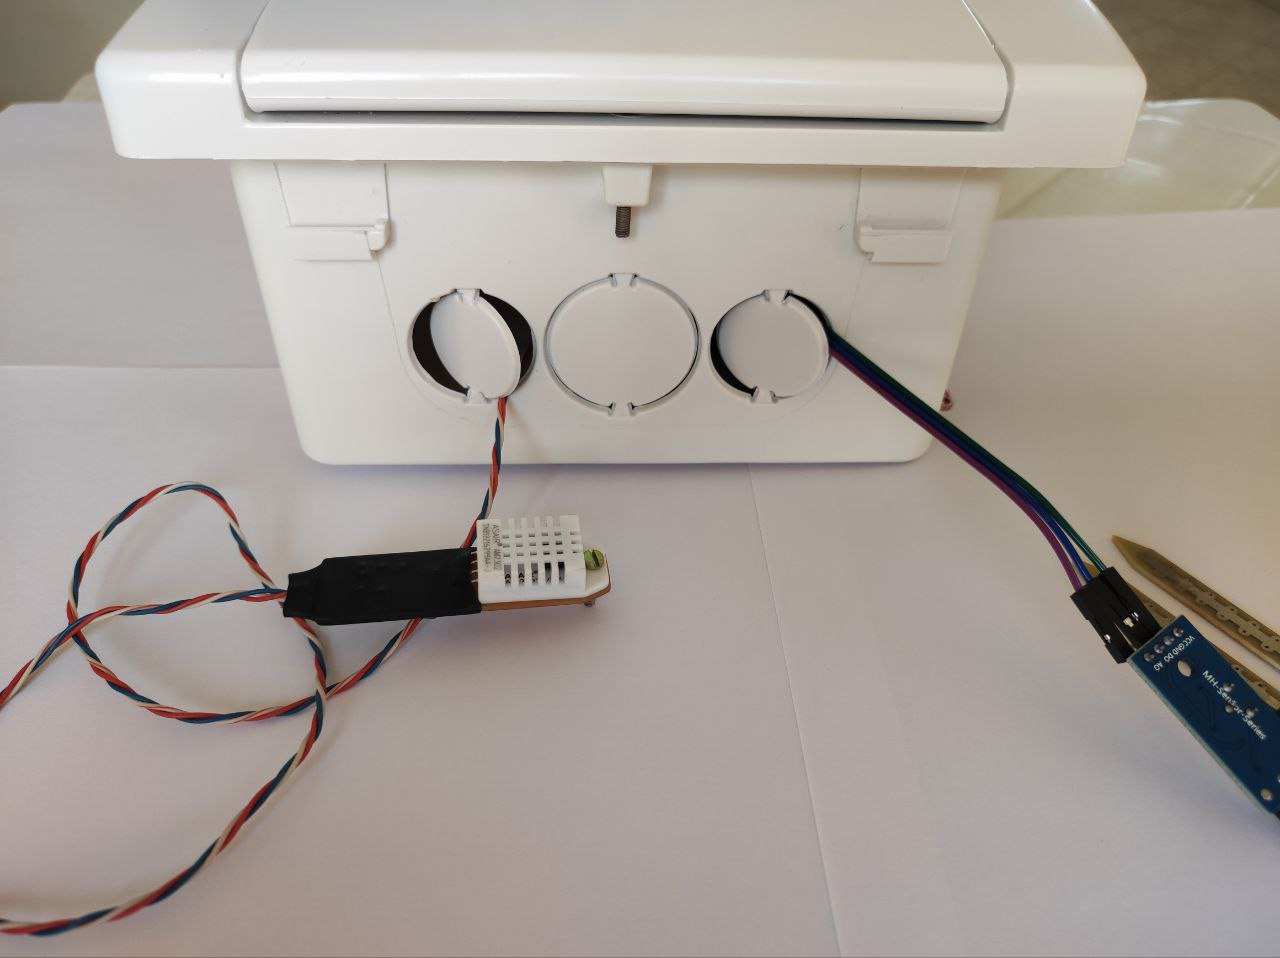
\includegraphics[width=7cm]{figuras/saidasensores.jpg}\\
% 	\autoria{Autoria Própria}
% 	\label{fig:saidasensores}
% \end{figure}

% A Figura \ref{fig:prontos} apresenta o trabalho com sua montagem finalizada, tendo apenas a interface humano/máquina disponível ao usuário, tornando o sistema mais amigável para pessoas com pouca afinidade à sistema eletrônicos complexos. O sistema pode ser fixado facilmente em paredes, estruturas de madeira, metal ou outro material que possa ser usado para construção de estrutura de estufa. A tampa de proteção inibe que os botões sejam acionados acidentalmente, além de proteger a IHM de fatores externos.

% \begin{figure}[!h]
% 	\centering
% 	\caption{Sistema finalizado}
% 	%\vskip 5mm
% 	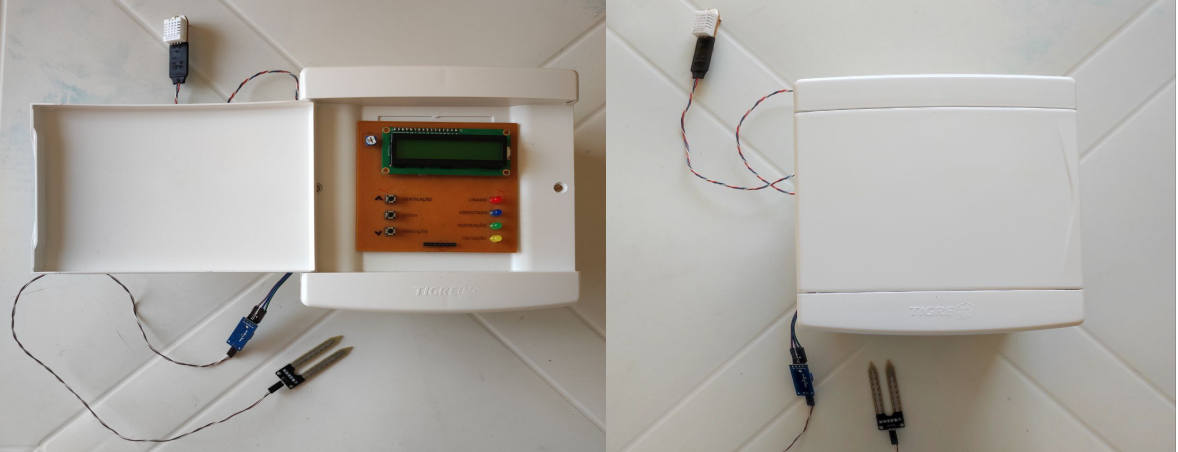
\includegraphics[width=12cm]{figuras/prontos.png}\\
% 	\autoria{Autoria Própria}
% 	\label{fig:prontos}
% \end{figure}

% Para a realização dos testes práticos, o sistema foi configurado, através da IHM física, para o plantio de coentro, como apresentado na Figura \ref{fig:coentro}. Desse modo, o sistema assumiu os valores de temperatura e umidade do solo utilizado programados para o coentro.   

% \begin{figure}[!h]
% 	\centering
% 	\caption{Configuração do sistema para o plantio de coentro}
% 	%\vskip 5mm
% 	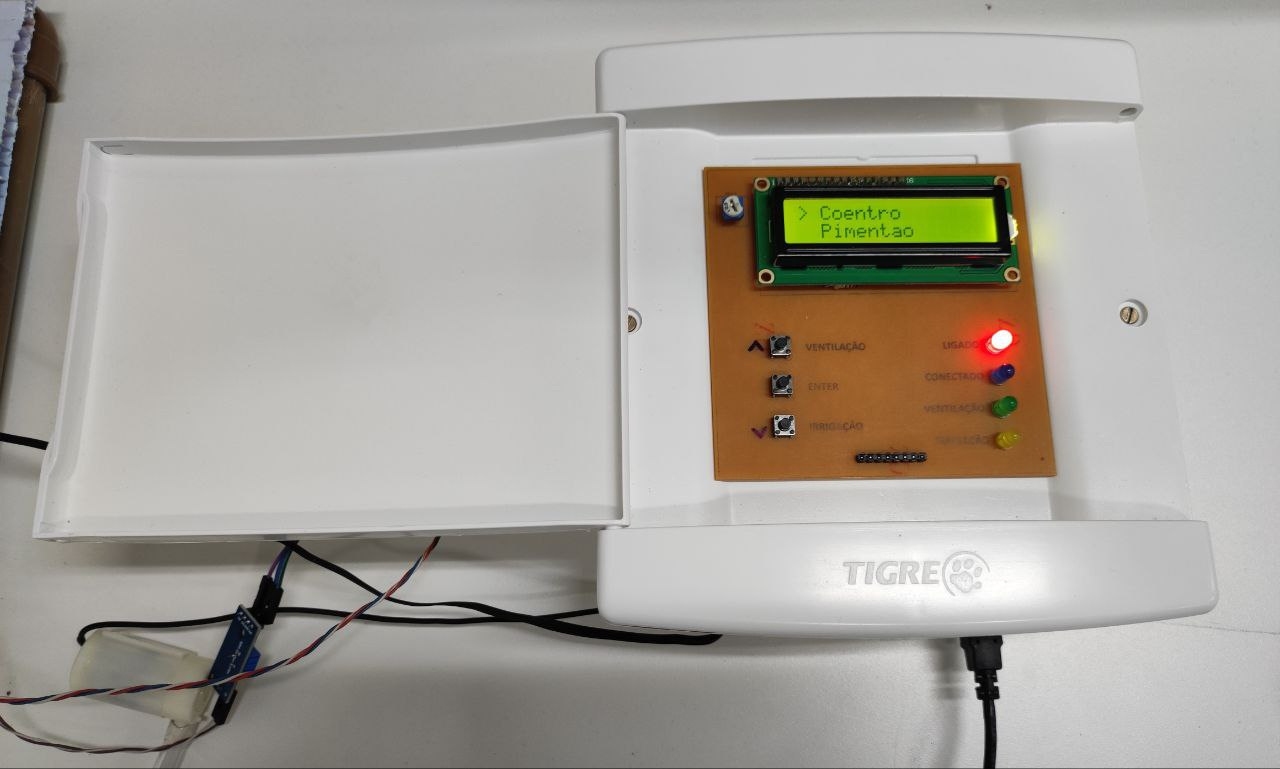
\includegraphics[width=10cm]{figuras/coentro.jpg}\\
% 	\autoria{Autoria Própria}
% 	\label{fig:coentro}
% \end{figure}

% Após a configuração, os testes realizados utilizaram os valores apresentados na Tabela \ref{tab:parametros}. O sistema tinha como propósito manter a temperatura e umidade do solo entre a faixa estabelecia, devendo acionar e desacionar a irrigação e o sistema de ventilação sempre que necessário e até o valor se encontrar dentro da faixa, respeitando a programação apresentada no capítulo anterior.

% \begin{table}[!h]
% \centering
% \caption{Valores limites para temperatura e umidade do solo}
% \label{tab:parametros}
% \begin{tabular}{c|c|c}
% \hline
% Descrição & Mínimo & Máximo \\ \hline
% Temperatura & 25°C & 35°C \\ \hline
% \begin{tabular}[c]{@{}c@{}}Umidade do\\ solo\end{tabular} & 45\% & 65\% \\ \hline
% \end{tabular}
% \\
% \autoria{Autoria própria}
% \end{table}

% Para a realização dos testes foi desenvolvida estrutura para simular um ambiente de estufa utilizando materiais plásticos. Na Figura~\ref{fig:mont1} é ilustrado o protótipo em fase de desenvolvimento, em que pode-se observar o ventilador ao fundo. 

% \begin{figure}[!h]
% 	\centering
% 	\caption{Estrutura parcial}
% 	%\vskip 5mm
% 	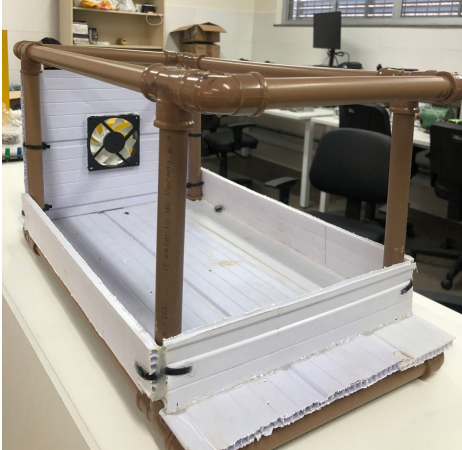
\includegraphics[width=8cm]{figuras/montagem1.png}\\
% 	\autoria{Autoria Própria}
% 	\label{fig:mont1}
% \end{figure}

% Na Figura~\ref{fig:mont2} é observada a estrutura finalizada, contendo em seu interior os sensores de temperatura e umidade do ar, além do sensor de umidade do solo e, ao lado, reservatório contendo água e a bomba submersa.

% \begin{figure}[!h]
% 	\centering
% 	\caption{Estrutura finalizada}
% 	%\vskip 5mm
% 	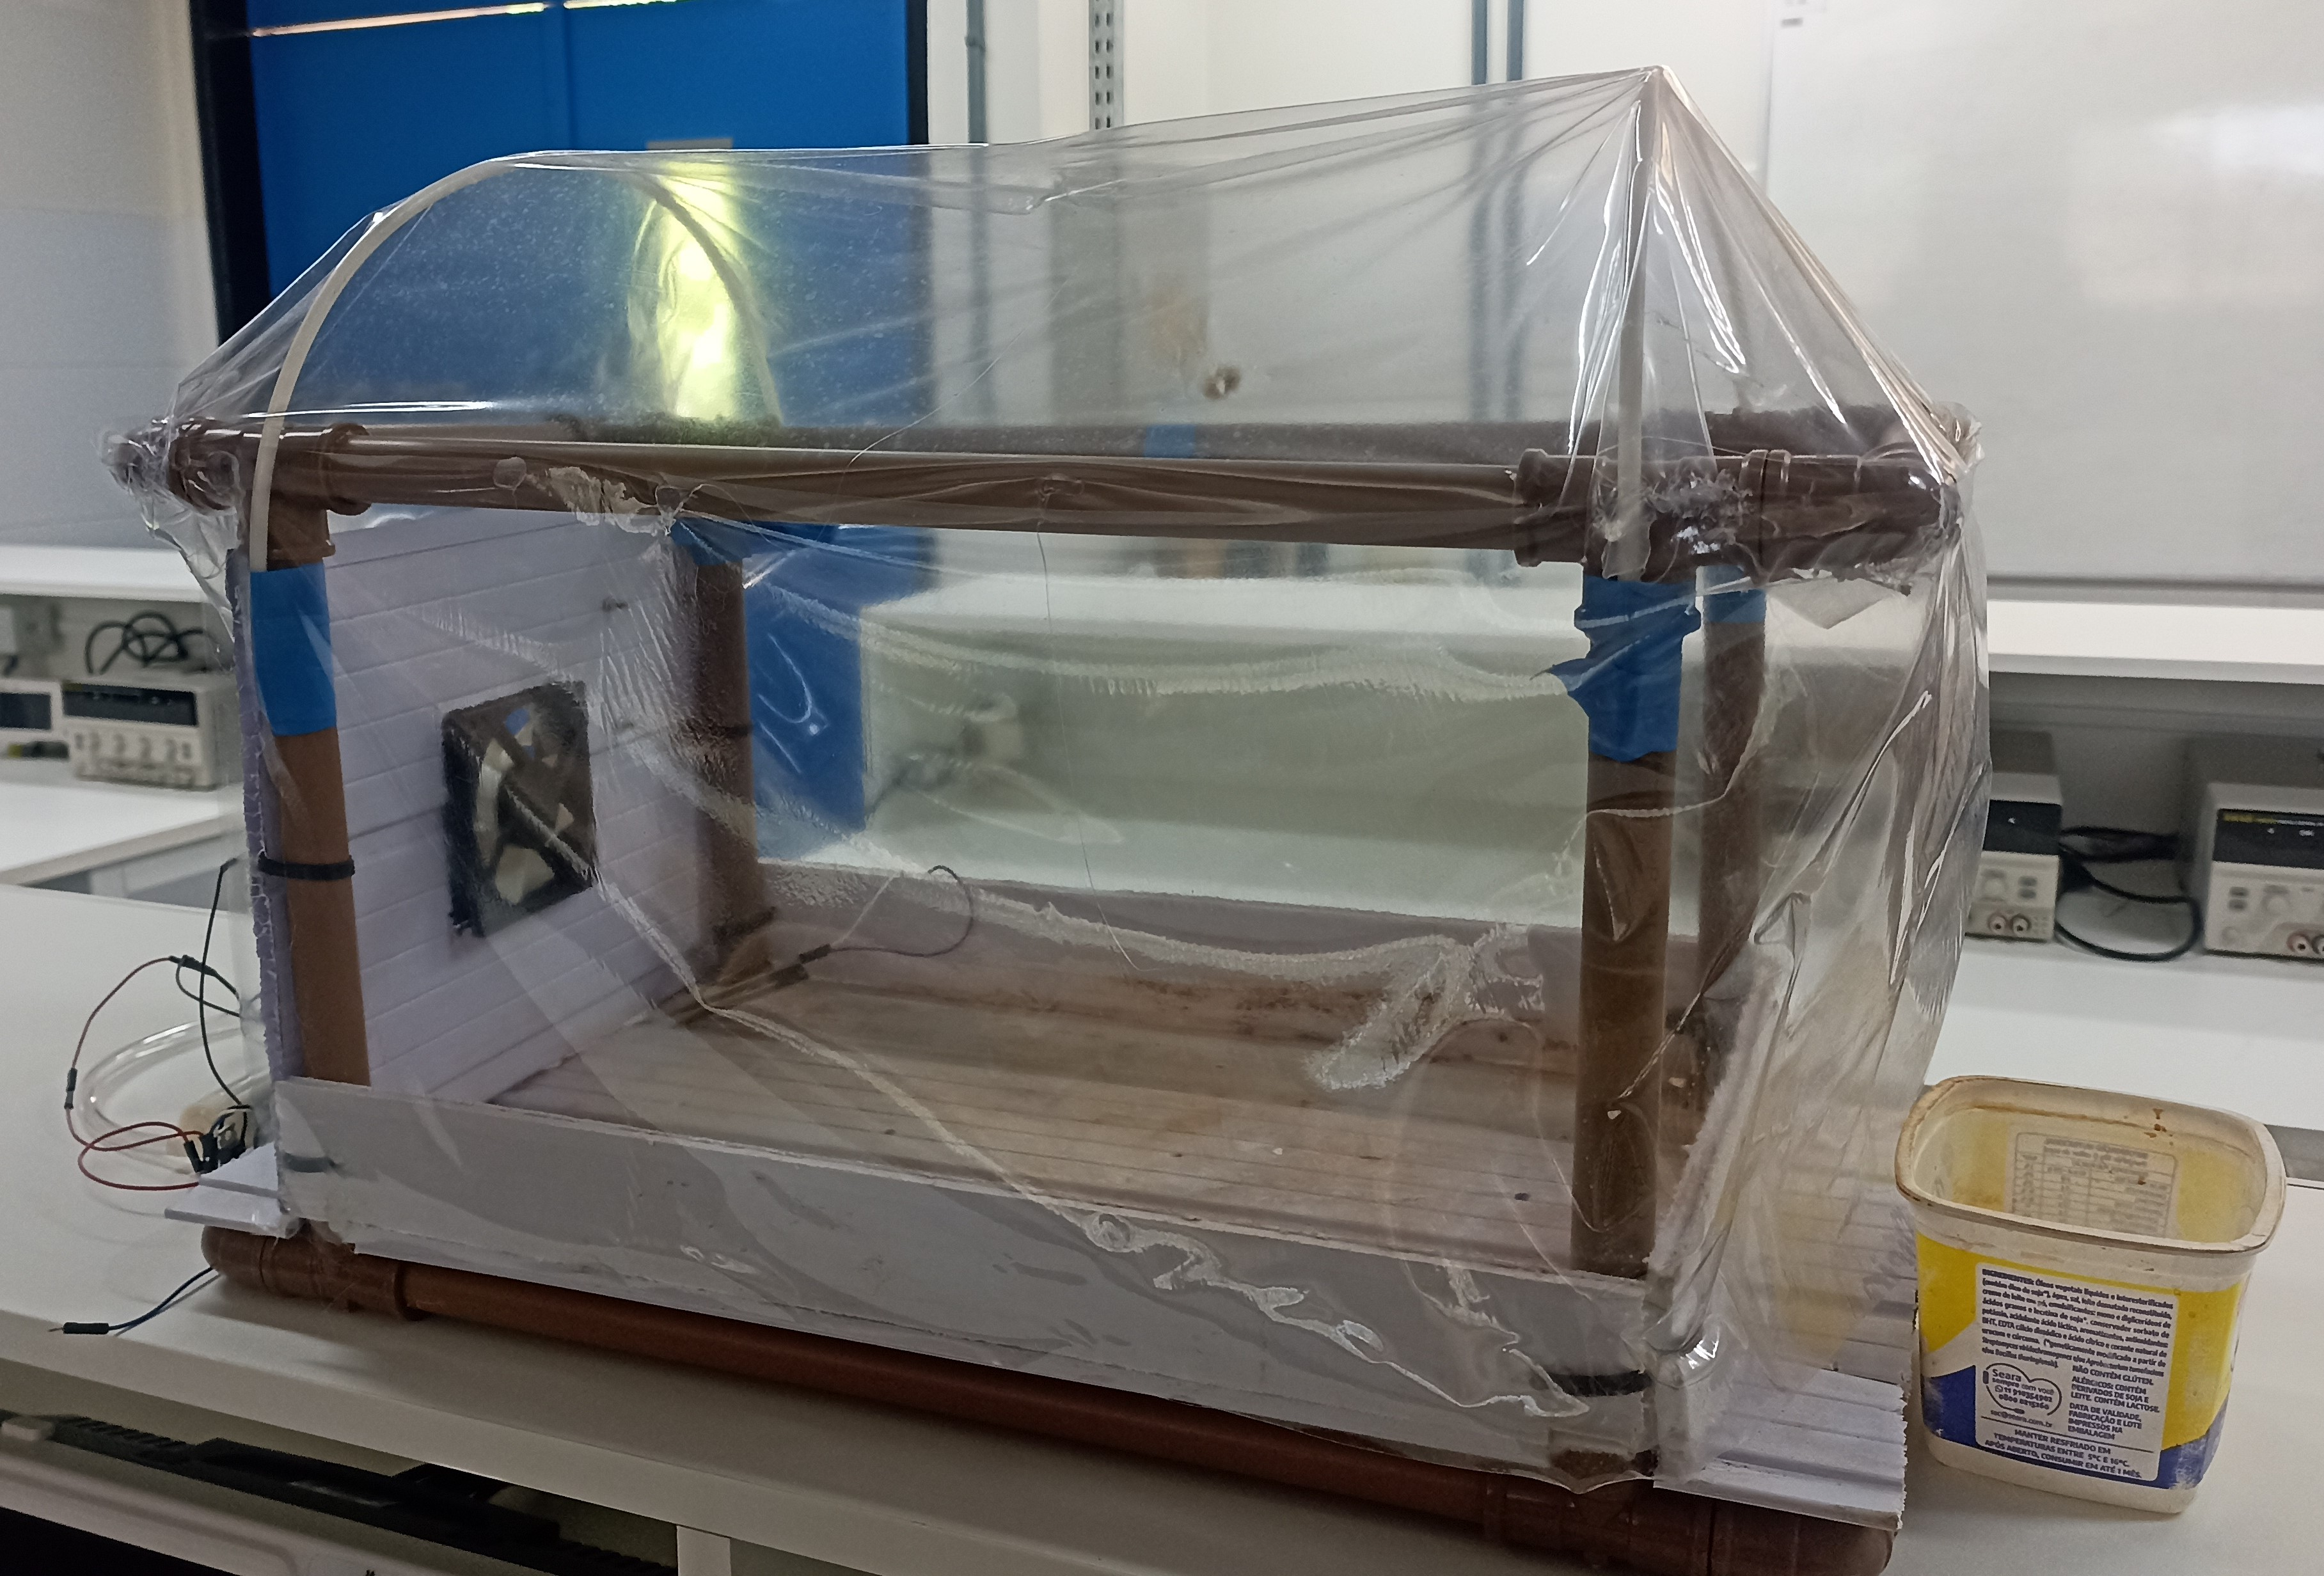
\includegraphics[width=8cm]{figuras/estufapronta.jpg}\\
% 	\autoria{Autoria Própria}
% 	\label{fig:mont2}
% \end{figure}

% Ao início dos testes, as condições iniciais foram de solo totalmente seco e temperatura ambiente em local externo, exposto ao sol, com temperatura interna à estufa em 38°C, visando simular as condições reais de uma estufa agrícola. Os testes foram realizados ao longo de 4 horas contínuas, onde foram aferidos os valores a cada 5 minutos. 


% Como o solo se apresentava seco, o sistema acionou a irrigação, onde pode-se observar na Figura \ref{fig:graficoumidadesolo} a elevação da umidade do solo até ser atingido o valor estipulado pela programação. No momento em que a umidade do solo atingiu o valor, a irrigação foi desligada, no decorrer do teste, o valor de umidade reduziu gradativamente, por conta da evaporação natural, ao atingir o valor mínimo, a irrigação foi novamente acionada, mantendo o nível sempre na faixa estipulada.

% \begin{figure}[!h]
% 	\centering
% 	\caption{Variação da umidade do solo}
% 	%\vskip 5mm
% 	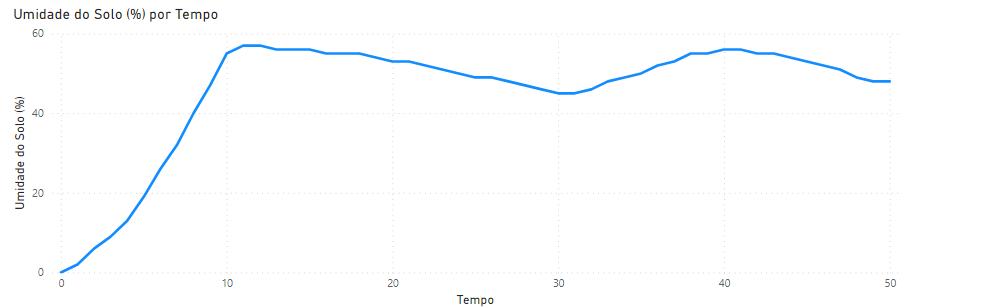
\includegraphics[width=16cm]{figuras/graficoumidadesolo.png}\\
% 	\autoria{Autoria Própria}
% 	\label{fig:graficoumidadesolo}
% \end{figure}

% De acordo com a variação da umidade do solo, o sistema realizou o controle do módulo atuador, onde o estado da bomba de irrigação é apresentado na Figura \ref{fig:graficoirrig}. Nota-se que o acionamento da irrigação foi realizado apenas quando necessário, evitando o uso desnecessário de água. Foi possível observar a eficácia da programação orientada a evitar o acionamento indevido em torno dos valores limites, evitando a danificação do equipamento.

% \begin{figure}[!h]
% 	\centering
% 	\caption{Variação do estado da irrigação}
% 	%\vskip 5mm
% 	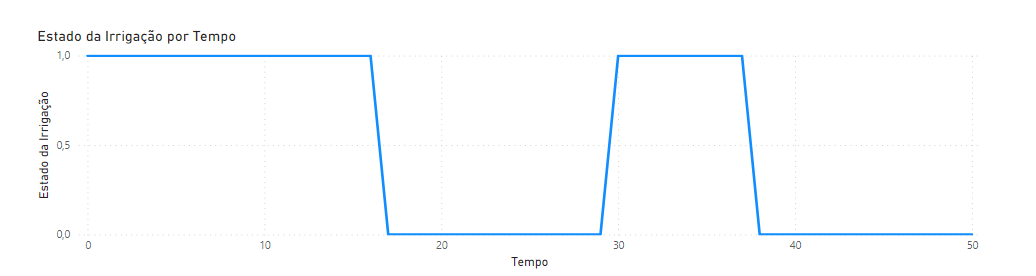
\includegraphics[width=16cm]{figuras/graficoestadoirrig.png}\\
% 	\autoria{Autoria Própria}
% 	\label{fig:graficoirrig}
% \end{figure}

% A variação da temperatura durante o teste ocorreu de maneira lenta e gradativa, devido ao ventilador usado ser de baixa potência, porém, O sistema foi capaz de manter o valor dentro da faixa estipulada em programação para o cultivo de coentro. A Figura \ref{fig:temp} apresenta a variação da temperatura medida pelo sensor, nota-se que inicialmente a temperatura estava acima da faixa ideal, sendo imediatamente acionada a ventilação. O sistema foi programado para reduzir a temperatura até o limite mínimo definido, visando aumentar o tempo em que o sistema permanece no valor ideal, sem que haja a necessidade da ventilação permanecer acionada. 

% \begin{figure}[!h]
% 	\centering
% 	\caption{Variação da temperatura}
% 	%\vskip 5mm
% 	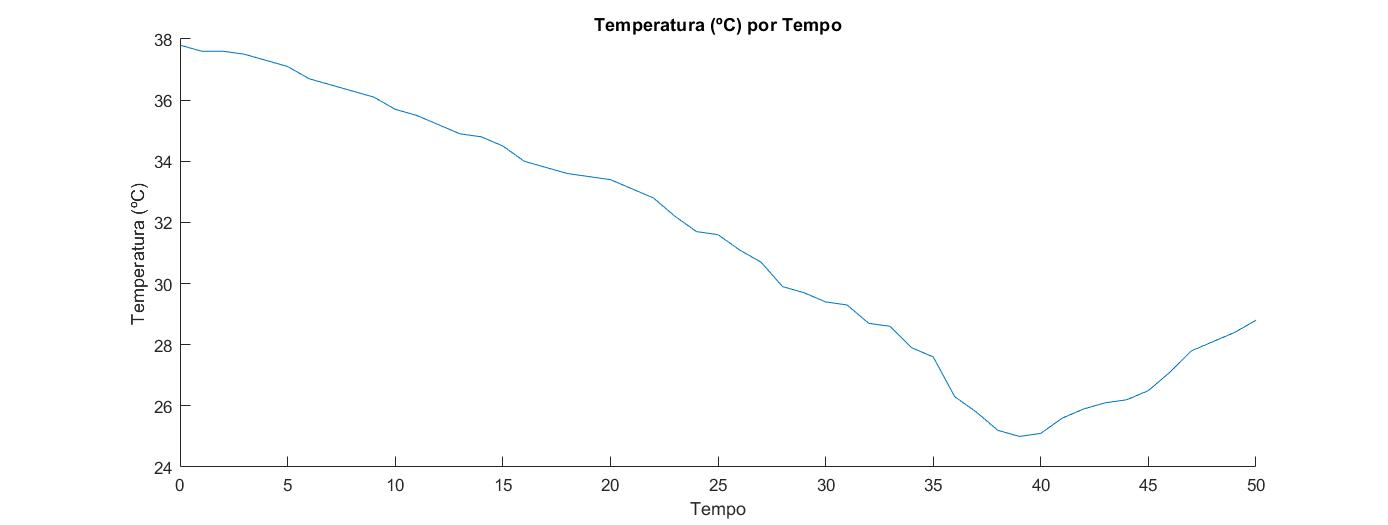
\includegraphics[width=16cm]{figuras/graficotemp.jpg}\\
% 	\autoria{Autoria Própria}
% 	\label{fig:temp}
% \end{figure}

% Do mesmo modo que o acionamento da irrigação, a ventilação foi acionada apenas quando necessário, até que a temperatura atingisse o nível estipulado. A Figura \ref{fig:estv} apresenta o estado do ventilador ao longo do teste. ao analisar os dados apresentados, é possível prever o comportamento do sistema de ventilação de acordo com a média de temperatura ambiente do local de instalação do sistema e também a faixa de temperatura ideal do plantio escolhido, permitindo escolher o melhor sistema de ventilação ou refrigeração a ser aplicado à estufa.

% \begin{figure}[!h]
% 	\centering
% 	\caption{Variação do estado da ventilação}
% 	%\vskip 5mm
% 	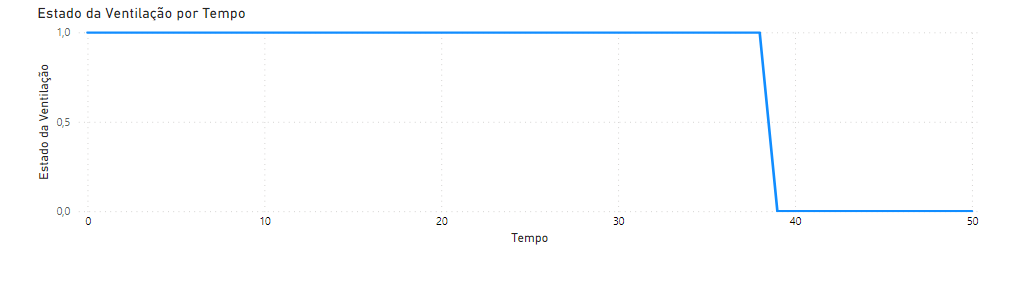
\includegraphics[width=16cm]{figuras/graficoestadovent.png}\\
% 	\autoria{Autoria Própria}
% 	\label{fig:estv}
% \end{figure}


% Desta forma, os testes comprovam a eficácia do sistema desenvolvido com relação ao controle e automação da irrigação. Vale destacar que a única intervenção necessária do usuário é na etapa de escolha do plantio, reduzindo o tempo e trabalho gastos durante o processo de irrigação. O sistema foi capaz de manter os níveis de temperatura e umidade do solo dentro da faixa ideal escolhida, permitindo a maximização da produção e reduzindo o uso de insumos agrícolas.